\documentclass[10pt,fleqn]{article} % Default font size and left-justified equations
\usepackage[%
    pdftitle={Modélisation cinématique : Chaîne ouverte},
    pdfauthor={Xavier Pessoles}]{hyperref}

%%%%%%%%%%%%%%%%%%%%%%%%%%%%%%%%%%%%%%%%%
% Original author:
% Mathias Legrand (legrand.mathias@gmail.com) with modifications by:
% Vel (vel@latextemplates.com)
% License:
% CC BY-NC-SA 3.0 (http://creativecommons.org/licenses/by-nc-sa/3.0/)
%%%%%%%%%%%%%%%%%%%%%%%%%%%%%%%%%%%%%%%%%

%----------------------------------------------------------------------------------------
%	VARIOUS REQUIRED PACKAGES AND CONFIGURATIONS
%----------------------------------------------------------------------------------------

%\usepackage[top=2.5cm,bottom=2cm,left=2cm,right=2cm,headsep=40pt,a4paper]{geometry} % Page margins
\usepackage[top=2cm,bottom=3cm,left=2cm,right=2cm,a4paper]{geometry} % Page margins

\usepackage{graphicx} % Required for including pictures

\usepackage{lipsum} % Inserts dummy text

\usepackage{tikz} % Required for drawing custom shapes

\usepackage[francais]{babel} % English language/hyphenation
\frenchbsetup{StandardLists=true} % Pour éviter la collision babel enumitem pour les listes

\usepackage{enumitem} % Customize lists
\setlist{nolistsep} % Reduce spacing between bullet points and numbered lists

\usepackage{booktabs} % Required for nicer horizontal rules in tables

\usepackage{xcolor} % Required for specifying colors by name
%\definecolor{ocre}{RGB}{243,102,25} % Define the orange color used for highlighting throughout the book
 \definecolor{ocre}{RGB}{49,133,156} % Couleur ''bleue''
\definecolor{violetf}{RGB}{112,48,160} % Couleur ''violet''
\usepackage{enumitem}
\usepackage{pifont} % Pour les dinglist
\usepackage{multicol}
\usepackage{array} % Centrage vertical dans les tableaux
\usepackage{schemabloc}

%----------------------------------------------------------------------------------------
%	FONTS
%----------------------------------------------------------------------------------------
\usepackage{bm}
\usepackage{multicol}
\usepackage{siunitx}
\sisetup{output-decimal-marker = {,}}


\usepackage{avant} % Use the Avantgarde font for headings
%\usepackage{times} % Use the Times font for headings
%\usepackage{mathptmx} % Use the Adobe Times Roman as the default text font together with math symbols from the Sym­bol, Chancery and Com­puter Modern fonts
\usepackage[adobe-utopia]{mathdesign}
\usepackage{microtype} % Slightly tweak font spacing for aesthetics
\usepackage[utf8]{inputenc} % Required for including letters with accents
\usepackage[T1]{fontenc} % Use 8-bit encoding that has 256 glyphs

%----------------------------------------------------------------------------------------
%	BIBLIOGRAPHY AND INDEX
%----------------------------------------------------------------------------------------

%\usepackage[style=alphabetic,citestyle=numeric,sorting=nyt,sortcites=true,autopunct=true,babel=hyphen,hyperref=true,abbreviate=false,backref=true,backend=biber]{biblatex}
\usepackage[style=alphabetic,citestyle=numeric,sorting=nyt,sortcites=true,autopunct=true,hyperref=true,abbreviate=false,backref=true,backend=biber]{biblatex}
\addbibresource{bibliography.bib} % BibTeX bibliography file
\defbibheading{bibempty}{}

\usepackage{calc} % For simpler calculation - used for spacing the index letter headings correctly
\usepackage{makeidx} % Required to make an index
\makeindex % Tells LaTeX to create the files required for indexing

%----------------------------------------------------------------------------------------
%	MAIN TABLE OF CONTENTS
%----------------------------------------------------------------------------------------

\usepackage{titletoc} % Required for manipulating the table of contents

\setcounter{tocdepth}{2}     % Dans la table des matieres
\setcounter{secnumdepth}{2}

\contentsmargin{0cm} % Removes the default margin

% Part text styling
\titlecontents{part}[0cm]
{\addvspace{20pt}\centering\large\bfseries}
{}
{}
{}

% Chapter text styling
\titlecontents{chapter}[1.25cm] % Indentation
{\addvspace{12pt}\large\sffamily\bfseries} % Spacing and font options for chapters
{\color{ocre!60}\contentslabel[\Large\thecontentslabel]{1.25cm}\color{ocre}} % Chapter number
{\color{ocre}}  
{\color{ocre!60}\normalsize\;\titlerule*[.5pc]{.}\;\thecontentspage} % Page number

% Section text styling
\titlecontents{section}[1.25cm] % Indentation
{\addvspace{3pt}\sffamily\bfseries} % Spacing and font options for sections
{\color{ocre!60}\contentslabel[\thecontentslabel]{1.25cm} \color{ocre}} % Section number
{\color{ocre}}
{\hfill\color{ocre!60}\thecontentspage} % Page number
[]

% Subsection text styling
\titlecontents{subsection}[1.25cm] % Indentation
{\addvspace{1pt}\sffamily\small} % Spacing and font options for subsections
{\contentslabel[\thecontentslabel]{1.25cm}} % Subsection number
{}
{\ \titlerule*[.5pc]{.}\;\thecontentspage} % Page number
[]


% Subsection text styling
\titlecontents{subsubsection}[1.25cm] % Indentation
{\addvspace{1pt}\sffamily\small} % Spacing and font options for subsections
{\contentslabel[\thecontentslabel]{1.25cm}} % Subsection number
{}
{\ \titlerule*[.5pc]{.}\;\thecontentspage} % Page number
[]

% List of figures
\titlecontents{figure}[0em]
{\addvspace{-5pt}\sffamily}
{\thecontentslabel\hspace*{1em}}
{}
{\ \titlerule*[.5pc]{.}\;\thecontentspage}
[]

% List of tables
\titlecontents{table}[0em]
{\addvspace{-5pt}\sffamily}
{\thecontentslabel\hspace*{1em}}
{}
{\ \titlerule*[.5pc]{.}\;\thecontentspage}
[]

%----------------------------------------------------------------------------------------
%	MINI TABLE OF CONTENTS IN PART HEADS
%----------------------------------------------------------------------------------------

% Chapter text styling
\titlecontents{lchapter}[0em] % Indenting
{\addvspace{15pt}\large\sffamily\bfseries} % Spacing and font options for chapters
{\color{ocre}\contentslabel[\Large\thecontentslabel]{1.25cm}\color{ocre}} % Chapter number
{}  
{\color{ocre}\normalsize\sffamily\bfseries\;\titlerule*[.5pc]{.}\;\thecontentspage} % Page number

% Section text styling
\titlecontents{lsection}[0em] % Indenting
{\sffamily\small} % Spacing and font options for sections
{\contentslabel[\thecontentslabel]{1.25cm}} % Section number
{}
{}

% Subsection text styling
\titlecontents{lsubsection}[.5em] % Indentation
{\normalfont\footnotesize\sffamily} % Font settings
{}
{}
{}

%----------------------------------------------------------------------------------------
%	PAGE HEADERS
%----------------------------------------------------------------------------------------

\usepackage{fancyhdr} % Required for header and footer configuration



\pagestyle{fancy}
 \renewcommand{\headrulewidth}{0pt}
 \fancyhead{}
 
 % ENTETES de page
 \fancyhead[L]{%
 \noindent\begin{minipage}[c]{2.6cm}%
 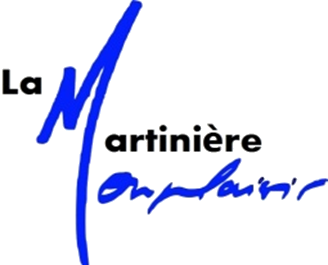
\includegraphics[width=2cm]{logo_lycee.png}%
 \end{minipage}
}

\fancyhead[C]{\rule{8cm}{.5pt}}

 \fancyhead[R]{%
 \noindent\begin{minipage}[c]{3cm}
 \begin{flushright}
 \footnotesize{\textit{\textsf{\xxtete}}}%
 \end{flushright}
 \end{minipage}
}

 \fancyfoot{}
 % PIEDS de page
\fancyfoot[C]{\rule{12cm}{.5pt}}
\renewcommand{\footrulewidth}{0.2pt}
\fancyfoot[C]{\footnotesize{\bfseries \thepage}}
\fancyfoot[L]{ 
\begin{minipage}[c]{.4\linewidth}
\noindent\footnotesize{{\xxauteur}}
\end{minipage}}

\fancyfoot[R]{\footnotesize{\xxpied}
\ifthenelse{\isodd{\value{page}}}{
\begin{tikzpicture}[overlay]
\node[shape=rectangle, 
      rounded corners = .25 cm,
	  draw= ocre,
	  line width=2pt, 
	  fill = ocre!10,
	  minimum width  = 2.5cm,
	  minimum height = 3cm,] at (\xxposongletx,\xxposonglety) {};
\node at (\xxposonglettext,\xxposonglety) {\rotatebox{90}{\textbf{\large\color{ocre}{\xxonglet}}}};
%{};
\end{tikzpicture}}{}
}



%
%
%
% Removes the header from odd empty pages at the end of chapters
\makeatletter
%\renewcommand{\cleardoublepage}{
%\clearpage\ifodd\c@page\else
%\hbox{}
%\vspace*{\fill}
%\thispagestyle{empty}
%\newpage
%\fi}

%\fancypagestyle{plain}{%
%\fancyhf{} % vide l’en-tête et le pied~de~page.
%%\fancyfoot[C]{\bfseries \thepage} % numéro de la page en cours en gras
%% et centré en pied~de~page.
%\fancyfoot[R]{\footnotesize{\xxpied}}
%\fancyfoot[C]{\rule{12cm}{.5pt}}
%\renewcommand{\footrulewidth}{0.2pt}
%\fancyfoot[C]{\footnotesize{\bfseries \thepage}}
%\fancyfoot[L]{ 
%\begin{minipage}[c]{.4\linewidth}
%\noindent\footnotesize{{\xxauteur}}
%\end{minipage}}}

\fancypagestyle{plain}{%
\fancyhf{} % vide l’en-tête et le pied~de~page.
\fancyfoot[C]{\rule{12cm}{.5pt}}
\renewcommand{\footrulewidth}{0.2pt}
\fancyfoot[C]{\footnotesize{\bfseries \thepage}}
\fancyfoot[L]{ 
\begin{minipage}[c]{.4\linewidth}
\noindent\footnotesize{{\xxauteur}}
\end{minipage}}
\fancyfoot[R]{\footnotesize{\xxpied}}
}




%----------------------------------------------------------------------------------------
%	THEOREM STYLES
%----------------------------------------------------------------------------------------

% Conflit avec la police adobe
%\usepackage{amsmath,amsfonts,amssymb,amsthm} % For math equations, theorems, symbols, etc
\usepackage{amsmath,amsthm}

\newcommand{\intoo}[2]{\mathopen{]}#1\,;#2\mathclose{[}}
\newcommand{\ud}{\mathop{\mathrm{{}d}}\mathopen{}}
\newcommand{\intff}[2]{\mathopen{[}#1\,;#2\mathclose{]}}
%\newtheorem{notation}{Notation}[chapter]
\newtheorem{notation}{Notation}[section]

% Boxed/framed environments
\newtheoremstyle{ocrenumbox}% % Theorem style name
{0pt}% Space above
{0pt}% Space below
{\normalfont}% % Body font
{}% Indent amount
{\small\bf\sffamily\color{ocre}}% % Theorem head font
{\;}% Punctuation after theorem head
{0.25em}% Space after theorem head
{\small\sffamily\color{ocre}\thmname{#1}\nobreakspace\thmnumber%{\@ifnotempty{#1}{}\@upn{#2}}% Theorem text (e.g. Theorem 2.1)
\thmnote{\nobreakspace\the\thm@notefont\sffamily\bfseries\color{black}---\nobreakspace#3.}} % Optional theorem note
\renewcommand{\qedsymbol}{$\blacksquare$}% Optional qed square


% Boite pour les corriges
\newtheoremstyle{correctionbox}% % Theorem style name
{0pt}% Space above
{0pt}% Space below
{\normalfont}% % Body font
{}% Indent amount
{\small\bf\sffamily\color{violet}}% % Theorem head font
{\;}% Punctuation after theorem head
{0.25em}% Space after theorem head
{\small\sffamily\color{ocre}\thmname{#1}\nobreakspace\thmnumber%{\@ifnotempty{#1}{}\@upn{#2}}% Theorem text (e.g. Theorem 2.1)
\thmnote{\nobreakspace\the\thm@notefont\sffamily\bfseries\color{black}---\nobreakspace#3.}} % Optional theorem note
\renewcommand{\qedsymbol}{$\blacksquare$}% Optional qed square



\newtheoremstyle{blacknumex}% Theorem style name
{5pt}% Space above
{5pt}% Space below
{\normalfont}% Body font
{} % Indent amount
{\small\bf\sffamily}% Theorem head font
{\;}% Punctuation after theorem head
{0.25em}% Space after theorem head
{\small\sffamily{\tiny\ensuremath{\blacksquare}}\nobreakspace\thmname{#1}\nobreakspace\thmnumber%{\@ifnotempty{#1}{}\@upn{#2}}% Theorem text (e.g. Theorem 2.1)
\thmnote{\nobreakspace\the\thm@notefont\sffamily\bfseries---\nobreakspace#3.}}% Optional theorem note

\newtheoremstyle{blacknumbox} % Theorem style name
{0pt}% Space above
{0pt}% Space below
{\normalfont}% Body font
{}% Indent amount
{\small\bf\sffamily}% Theorem head font
{\;}% Punctuation after theorem head
{0.25em}% Space after theorem head
{\small\sffamily\thmname{#1}\nobreakspace 
\thmnote{\nobreakspace\the\thm@notefont\sffamily\bfseries---\nobreakspace#3.}}% Optional theorem note

% Non-boxed/non-framed environments
\newtheoremstyle{ocrenum}% % Theorem style name
{5pt}% Space above
{5pt}% Space below
{\normalfont}% % Body font
{}% Indent amount
{\small\bf\sffamily\color{ocre}}% % Theorem head font
{\;}% Punctuation after theorem head
{0.25em}% Space after theorem head
{\small\sffamily\color{ocre}\thmname{#1}\nobreakspace%\thmnumber{\@ifnotempty{#1}{}\@upn{#2}}% Theorem text (e.g. Theorem 2.1)
\thmnote{\nobreakspace\the\thm@notefont\sffamily\bfseries\color{black}---\nobreakspace#3.}} % Optional theorem note
\renewcommand{\qedsymbol}{$\blacksquare$}% Optional qed square
\makeatother

% Environnement pour les titres de parties
\newtheoremstyle{partiebox} 
{0pt}% Space above
{0pt}% Space below
{\normalfont}% Body font
{}% Indent amount
{\small\bf\sffamily}% Theorem head font
{\;}% Punctuation after theorem head
{0.25em}% Space after theorem head




% Defines the theorem text style for each type of theorem to one of the three styles above
\newcounter{dummy} 
\numberwithin{dummy}{section}
\theoremstyle{ocrenumbox}
%\newtheorem{theoremeT}[dummy]{Théorème}
\newtheorem{theoremeT}[dummy]{Théorème}
\newtheorem{resultatT}[dummy]{Résultat}
\newtheorem{savoirT}[dummy]{Savoir}
\newtheorem{methodeT}[dummy]{Méthode}
\newtheorem{objectifT}[dummy]{Objectif}
%\newtheorem{problem}{Problem}[chapter]
\newtheorem{problem}{Problem}[section]
%\newtheorem{exerciseT}{Exercise}[chapter]
\newtheorem{exerciseT}{Exercice}[section]

\theoremstyle{blacknumex}
%\newtheorem{exampleT}{Example}[chapter]
\newtheorem{exempleT}{Exemple}[section]
\newtheorem{termT}{Terminal\\}[section]
\newtheorem{pyT}{Python\\}[section]
\newtheorem{sciT}{Scilab\\}[section]
\newtheorem{pseudoT}{Pseudo Code\\}[section]
\newtheorem{sqlT}{SQL\\}[section]

\theoremstyle{blacknumbox}
%\newtheorem{vocabulary}{Vocabulary}[chapter]
\newtheorem{vocabulary}{Vocabulaire}[section]
%\newtheorem{definitionT}{Definition}[section]
\newtheorem{definitionT}{Définition}[section]
\newtheorem{rappelT}{Rappel}[section]
\newtheorem{demoT}{Démonstration}[section]
\newtheorem{corollaryT}[dummy]{Corollaire}
\newtheorem{hypoT}{Hypothèse(s)}

\theoremstyle{ocrenum}
\newtheorem{proposition}[dummy]{Proposition}

\theoremstyle{partiebox}
\newtheorem{titrepartieT}[]{}
\newtheorem{titrechapitreT}[]{}

\theoremstyle{correctionbox}
\newtheorem{correctionT}[dummy]{\color{violet}{Correction}}

%----------------------------------------------------------------------------------------
%	DEFINITION OF COLORED BOXES
%----------------------------------------------------------------------------------------

\RequirePackage[framemethod=tikz]{mdframed} % Required for creating the theorem, definition, exercise and corollary boxes

% Theorem box
\newmdenv[skipabove=7pt,
skipbelow=7pt,
backgroundcolor=ocre!10,
linecolor=ocre,
innerleftmargin=5pt,
innerrightmargin=5pt,
innertopmargin=5pt,
leftmargin=0cm,
rightmargin=0cm,
innerbottommargin=5pt]{tBox}


% Correction
\newmdenv[skipabove=7pt,
skipbelow=7pt,
backgroundcolor=violet!10,
linecolor=violet,
innerleftmargin=5pt,
innerrightmargin=5pt,
innertopmargin=5pt,
leftmargin=0cm,
rightmargin=0cm,
innerbottommargin=5pt]{coBox}


% Exercise box	  
\newmdenv[skipabove=7pt,
skipbelow=7pt,
rightline=false,
leftline=true,
topline=false,
bottomline=false,
backgroundcolor=ocre!10,
linecolor=ocre,
innerleftmargin=5pt,
innerrightmargin=5pt,
innertopmargin=5pt,
innerbottommargin=5pt,
leftmargin=0cm,
rightmargin=0cm,
linewidth=4pt]{eBox}	

% Definition box
\newmdenv[skipabove=7pt,
skipbelow=7pt,
rightline=false,
leftline=true,
topline=false,
bottomline=false,
backgroundcolor=ocre!10,
linecolor=ocre,
innerleftmargin=5pt,
innerrightmargin=5pt,
innertopmargin=0pt,
leftmargin=0cm,
rightmargin=0cm,
linewidth=4pt,
innerbottommargin=0pt]{dBox}	

% Demonstration box
\newmdenv[skipabove=7pt,
skipbelow=7pt,
rightline=false,
leftline=true,
topline=false,
bottomline=false,
%backgroundcolor=ocre!10,
linecolor=ocre,
innerleftmargin=5pt,
innerrightmargin=5pt,
innertopmargin=0pt,
leftmargin=0cm,
rightmargin=0cm,
linewidth=4pt,
innerbottommargin=0pt]{demoBox}	

% Corollary box
\newmdenv[skipabove=7pt,
skipbelow=7pt,
rightline=false,
leftline=true,
topline=false,
bottomline=false,
linecolor=gray,
backgroundcolor=black!5,
innerleftmargin=5pt,
innerrightmargin=5pt,
innertopmargin=5pt,
leftmargin=0cm,
rightmargin=0cm,
linewidth=4pt,
innerbottommargin=5pt]{cBox}


% Hypothèses
\newmdenv[skipabove=7pt,
skipbelow=7pt,
rightline=false,
leftline=true,
topline=false,
bottomline=false,
linecolor=gray,
backgroundcolor=black!5,
innerleftmargin=5pt,
innerrightmargin=5pt,
innertopmargin=5pt,
leftmargin=0cm,
rightmargin=0cm,
linewidth=4pt,
innerbottommargin=5pt]{hyBox}


% Boite pour le titre de la partie (pBox)
\newmdenv[skipabove=7pt,
skipbelow=7pt,
rightline=true,
leftline=false,
topline=false,
bottomline=false,
linecolor=ocre,
backgroundcolor=none,
innerleftmargin=5pt,
innerrightmargin=5pt,
innertopmargin=5pt,
leftmargin=0cm,
rightmargin=0cm,
linewidth=4pt,
innerbottommargin=5pt]{pBox}

% Boite pour le titre du chapitre (chBox)
\newmdenv[skipabove=7pt,
skipbelow=7pt,
rightline=false,
leftline=true,
topline=false,
bottomline=false,
linecolor=ocre,
%backgroundcolor=black!5,
innerleftmargin=5pt,
innerrightmargin=5pt,
innertopmargin=5pt,
leftmargin=0cm,
rightmargin=0cm,
linewidth=4pt,
innerbottommargin=5pt]{chBox}


% Boite pour les exemples
\newmdenv[skipabove=7pt,
skipbelow=7pt,
rightline=false,
leftline=true,
topline=false,
bottomline=false,
linecolor=gray,
backgroundcolor=white,
innerleftmargin=5pt,
innerrightmargin=5pt,
innertopmargin=5pt,
leftmargin=0cm,
rightmargin=0cm,
linewidth=4pt,
innerbottommargin=5pt]{exBox}

% Boite pour le terminal
\newmdenv[skipabove=7pt,
skipbelow=7pt,
rightline=false,
leftline=true,
topline=false,
bottomline=false,
linecolor=gray,
backgroundcolor=white,
innerleftmargin=5pt,
innerrightmargin=5pt,
innertopmargin=5pt,
leftmargin=0cm,
rightmargin=0cm,
linewidth=4pt,
innerbottommargin=5pt]{termBox}


% Boite pour Python
\newmdenv[skipabove=7pt,
skipbelow=7pt,
rightline=false,
leftline=true,
topline=false,
bottomline=false,
linecolor=gray,
backgroundcolor=white,
innerleftmargin=5pt,
innerrightmargin=5pt,
innertopmargin=0pt,
leftmargin=0cm,
rightmargin=0cm,
linewidth=4pt,
innerbottommargin=5pt]{pyBox}

% Boite pour scilab
\newmdenv[skipabove=7pt,
skipbelow=7pt,
rightline=false,
leftline=true,
topline=false,
bottomline=false,
linecolor=gray,
backgroundcolor=white,
innerleftmargin=5pt,
innerrightmargin=5pt,
innertopmargin=5pt,
leftmargin=0cm,
rightmargin=0cm,
linewidth=4pt,
innerbottommargin=5pt]{sciBox}


% Boite pour pseudo
\newmdenv[skipabove=7pt,
skipbelow=7pt,
rightline=false,
leftline=true,
topline=false,
bottomline=false,
linecolor=gray,
backgroundcolor=white,
innerleftmargin=5pt,
innerrightmargin=5pt,
innertopmargin=5pt,
leftmargin=0cm,
rightmargin=0cm,
linewidth=4pt,
innerbottommargin=5pt]{pseudoBox}

% Boite pour pseudo
\newmdenv[skipabove=7pt,
skipbelow=7pt,
rightline=false,
leftline=true,
topline=false,
bottomline=false,
linecolor=gray,
backgroundcolor=white,
innerleftmargin=5pt,
innerrightmargin=5pt,
innertopmargin=5pt,
leftmargin=0cm,
rightmargin=0cm,
linewidth=4pt,
innerbottommargin=5pt]{sqlBox}


% Creates an environment for each type of theorem and assigns it a theorem text style from the "Theorem Styles" section above and a colored box from above
\newenvironment{theorem}{\begin{tBox}\begin{theoremeT}}{\end{theoremeT}\end{tBox}}
\newenvironment{resultat}{\begin{tBox}\begin{resultatT}}{\end{resultatT}\end{tBox}}
\newenvironment{methode}{\begin{tBox}\begin{methodeT}}{\end{methodeT}\end{tBox}}
\newenvironment{savoir}{\begin{tBox}\begin{savoirT}}{\end{savoirT}\end{tBox}}
\newenvironment{obj}{\begin{tBox}\begin{objectifT}}{\end{objectifT}\end{tBox}}
\newenvironment{corrige}{\begin{coBox}\begin{correctionT}}{\end{correctionT}\end{coBox}}
\newenvironment{exercise}{\begin{eBox}\begin{exerciseT}}{\hfill{\color{ocre}\tiny\ensuremath{\blacksquare}}\end{exerciseT}\end{eBox}}				  
\newenvironment{exercice}{\begin{eBox}\begin{exerciseT}}{\hfill{\color{ocre}\tiny\ensuremath{\blacksquare}}\end{exerciseT}\end{eBox}}				  

\newenvironment{definition}{\begin{dBox}\begin{definitionT}}{\end{definitionT}\end{dBox}}	
\newenvironment{rappel}{\begin{dBox}\begin{rappelT}}{\end{rappelT}\end{dBox}}	
\newenvironment{defi}{\begin{dBox}\begin{definitionT}}{\end{definitionT}\end{dBox}}	
\newenvironment{demo}{\begin{demoBox}\begin{demoT}}{\end{demoT}\end{demoBox}}	
%\newenvironment{exemple}{\begin{exempleT}}{\hfill{\tiny\ensuremath{\blacksquare}}\end{exempleT}}		
\newenvironment{corollary}{\begin{cBox}\begin{corollaryT}}{\end{corollaryT}\end{cBox}}
\newenvironment{hypo}{\begin{hyBox}\begin{hypoT}}{\end{hypoT}\end{hyBox}}	\newenvironment{exemple}{\begin{exBox}\begin{exempleT}}{\hfill{\tiny\ensuremath{\blacksquare}}\end{exempleT}\end{exBox}}	
\newenvironment{titrepartie}{\begin{pBox}\begin{titrepartieT}}{\end{titrepartieT}\end{pBox}}	
\newenvironment{titrechapitre}{\begin{chBox}\begin{titrechapitreT}}{\end{titrechapitreT}\end{chBox}}	

\newenvironment{term}{ \begin{termBox}\begin{termT}}{\end{termT}\end{termBox}}
\newenvironment{py}{ \begin{pyBox}\begin{pyT}}{\end{pyT}\end{pyBox}}
\newenvironment{sci}{ \begin{sciBox}\begin{sciT}}{\end{sciT}\end{sciBox}}
\newenvironment{pseudo}{ \begin{pseudoBox}\begin{pseudoT}}{\end{pseudoT}\end{pseudoBox}}
\newenvironment{envsql}{ \begin{sqlBox}\begin{sqlT}}{\end{sqlT}\end{sqlBox}}


%----------------------------------------------------------------------------------------
%	REMARK ENVIRONMENT
%----------------------------------------------------------------------------------------

\newenvironment{remark}{\par\vspace{10pt}\small % Vertical white space above the remark and smaller font size
\begin{list}{}{
\leftmargin=35pt % Indentation on the left
\rightmargin=25pt}\item\ignorespaces % Indentation on the right
\makebox[-2.5pt]{\begin{tikzpicture}[overlay]
\node[draw=ocre!60,line width=1pt,circle,fill=ocre!25,font=\sffamily\bfseries,inner sep=2pt,outer sep=0pt] at (-15pt,0pt){\textcolor{ocre}{R}};\end{tikzpicture}} % Orange R in a circle
\advance\baselineskip -1pt}{\end{list}\vskip5pt} % Tighter line spacing and white space after remark

\newenvironment{rem}{\par\vspace{10pt}\small % Vertical white space above the remark and smaller font size
\begin{list}{}{
\leftmargin=35pt % Indentation on the left
\rightmargin=25pt}\item\ignorespaces % Indentation on the right
\makebox[-2.5pt]{\begin{tikzpicture}[overlay]
\node[draw=ocre!60,line width=1pt,circle,fill=ocre!25,font=\sffamily\bfseries,inner sep=2pt,outer sep=0pt] at (-15pt,0pt){\textcolor{ocre}{R}};\end{tikzpicture}} % Orange R in a circle
\advance\baselineskip -1pt}{\end{list}\vskip5pt} % Tighter line spacing and white space after remark


\newenvironment{warn}{\par\vspace{10pt}\small % Vertical white space above the remark and smaller font size
\begin{list}{}{
\leftmargin=35pt % Indentation on the left
\rightmargin=25pt}\item\ignorespaces % Indentation on the right
\makebox[-2.5pt]{\begin{tikzpicture}[overlay]
\node[draw=red!60,line width=1pt,circle,fill=red!25,font=\sffamily\bfseries,inner sep=2pt,outer sep=0pt] at (-15pt,0pt){\textcolor{black}{!}};\end{tikzpicture}} % Point d'exclamation dans un cercle
\advance\baselineskip -1pt}{\end{list}\vskip5pt} % Tighter line spacing and white space after remark


%----------------------------------------------------------------------------------------
%	SECTION NUMBERING IN THE MARGIN
%----------------------------------------------------------------------------------------
\setcounter{secnumdepth}{3}
\setcounter{tocdepth}{2}



\makeatletter
\renewcommand{\@seccntformat}[1]{\llap{\textcolor{ocre}{\csname the#1\endcsname}\hspace{1em}}}                    
\renewcommand{\section}{\@startsection{section}{1}{\z@}
{-4ex \@plus -1ex \@minus -.4ex}
{1ex \@plus.2ex }
{\normalfont\large\sffamily\bfseries}}
\renewcommand{\subsection}{\@startsection {subsection}{2}{\z@}
{-3ex \@plus -0.1ex \@minus -.4ex}
{0.5ex \@plus.2ex }
{\normalfont\sffamily\bfseries}}
\renewcommand{\subsubsection}{\@startsection {subsubsection}{3}{\z@}
{-2ex \@plus -0.1ex \@minus -.2ex}
{.2ex \@plus.2ex }
{\normalfont\small\sffamily\bfseries}}                        
\renewcommand\paragraph{\@startsection{paragraph}{4}{\z@}
{-2ex \@plus-.2ex \@minus .2ex}
{.1ex}
{\normalfont\small\sffamily\bfseries}}

%----------------------------------------------------------------------------------------
%	PART HEADINGS
%----------------------------------------------------------------------------------------


%----------------------------------------------------------------------------------------
%	CHAPTER HEADINGS
%----------------------------------------------------------------------------------------

% \newcommand{\thechapterimage}{}%
% \newcommand{\chapterimage}[1]{\renewcommand{\thechapterimage}{#1}}%
% \def\@makechapterhead#1{%
% {\parindent \z@ \raggedright \normalfont
% \ifnum \c@secnumdepth >\m@ne
% \if@mainmatter
% \begin{tikzpicture}[remember picture,overlay]
% \node at (current page.north west)
% {\begin{tikzpicture}[remember picture,overlay]
% \node[anchor=north west,inner sep=0pt] at (0,0) {\includegraphics[width=\paperwidth]{\thechapterimage}};
% \draw[anchor=west] (\Gm@lmargin,-9cm) node [line width=2pt,rounded corners=15pt,draw=ocre,fill=white,fill opacity=0.5,inner sep=15pt]{\strut\makebox[22cm]{}};
% \draw[anchor=west] (\Gm@lmargin+.3cm,-9cm) node {\huge\sffamily\bfseries\color{black}\thechapter. #1\strut};
% \end{tikzpicture}};
% \end{tikzpicture}
% \else
% \begin{tikzpicture}[remember picture,overlay]
% \node at (current page.north west)
% {\begin{tikzpicture}[remember picture,overlay]
% \node[anchor=north west,inner sep=0pt] at (0,0) {\includegraphics[width=\paperwidth]{\thechapterimage}};
% \draw[anchor=west] (\Gm@lmargin,-9cm) node [line width=2pt,rounded corners=15pt,draw=ocre,fill=white,fill opacity=0.5,inner sep=15pt]{\strut\makebox[22cm]{}};
% \draw[anchor=west] (\Gm@lmargin+.3cm,-9cm) node {\huge\sffamily\bfseries\color{black}#1\strut};
% \end{tikzpicture}};
% \end{tikzpicture}
% \fi\fi\par\vspace*{270\p@}}}

%-------------------------------------------

\def\@makeschapterhead#1{%
\begin{tikzpicture}[remember picture,overlay]
\node at (current page.north west)
{\begin{tikzpicture}[remember picture,overlay]
\node[anchor=north west,inner sep=0pt] at (0,0) {\includegraphics[width=\paperwidth]{\thechapterimage}};
\draw[anchor=west] (\Gm@lmargin,-9cm) node [line width=2pt,rounded corners=15pt,draw=ocre,fill=white,fill opacity=0.5,inner sep=15pt]{\strut\makebox[22cm]{}};
\draw[anchor=west] (\Gm@lmargin+.3cm,-9cm) node {\huge\sffamily\bfseries\color{black}#1\strut};
\end{tikzpicture}};
\end{tikzpicture}
\par\vspace*{270\p@}}
\makeatother

%----------------------------------------------------------------------------------------
%	HYPERLINKS IN THE DOCUMENTS
%----------------------------------------------------------------------------------------


\hypersetup{hidelinks,backref=true,pagebackref=true,hyperindex=true,colorlinks=false,breaklinks=true,urlcolor= ocre,bookmarks=true,bookmarksopen=false,pdftitle={Title},pdfauthor={Author}}
\usepackage{bookmark}
\bookmarksetup{
open,
numbered,
addtohook={%
\ifnum\bookmarkget{level}=0 % chapter
\bookmarksetup{bold}%
\fi
\ifnum\bookmarkget{level}=-1 % part
\bookmarksetup{color=ocre,bold}%
\fi
}
}

%----------------------------------------------------------------------------------------
%	
%----------------------------------------------------------------------------------------

\newcommand{\thechapterimage}{}%
\newcommand{\chapterimage}[1]{\renewcommand{\thechapterimage}{#1}}%
\def\@makechapterhead#1{%
{\parindent \z@ \raggedright \normalfont
\begin{tikzpicture}[remember picture,overlay]
\node at (current page.north west)
{\begin{tikzpicture}[remember picture,overlay]
\node[anchor=north west,inner sep=0pt] at (0,0) {\includegraphics[width=\paperwidth]{\thechapterimage}};
%\draw[anchor=west] (\Gm@lmargin,-9cm) node [line width=2pt,rounded corners=15pt,draw=ocre,fill=white,fill opacity=0.5,inner sep=15pt]{\strut\makebox[22cm]{}};
%\draw[anchor=west] (\Gm@lmargin+.3cm,-9cm) node {\huge\sffamily\bfseries\color{black}\thechapter. #1\strut};
\end{tikzpicture}};
\end{tikzpicture}
\par\vspace*{270\p@}
}}

 \newcounter{exo}


\makeatletter             
\renewcommand{\subparagraph}{\@startsection{exo}{5}{\z@}%
                                    {-2ex \@plus-.2ex \@minus .2ex}%
                                    {0ex}%               
{\normalfont\bfseries Question \hspace{.7cm} }}
\makeatother
\renewcommand{\thesubparagraph}{\arabic{subparagraph}} 
\makeatletter


\usepackage{textcomp}

% Définition des booleéns
\newif\iffiche
\newif\ifprof
\newif\iftd
\newif\ifcours
\newif\ifnormal
\newif\ifdifficile
\newif\iftdifficile
\newif\ifcolle
\newif\iflivret
%%%%%%%%%%%%
% Définition des vecteurs 
%%%%%%%%%%%%
\newcommand{\vect}[1]{\overrightarrow{#1}}
\newcommand{\axe}[2]{\left(#1,\vect{#2}\right)}
\newcommand{\couple}[2]{\left(#1,\vect{#2}\right)}
\newcommand{\angl}[2]{\left(\vect{#1},\vect{#2}\right)}

\newcommand{\rep}[1]{\mathcal{R}_{#1}}
\newcommand{\quadruplet}[4]{\left(#1;#2,#3,#4 \right)}
\newcommand{\repere}[4]{\left(#1;\vect{#2},\vect{#3},\vect{#4} \right)}
\newcommand{\base}[3]{\left(\vect{#1},\vect{#2},\vect{#3} \right)}


\newcommand{\vx}[1]{\vect{x_{#1}}}
\newcommand{\vy}[1]{\vect{y_{#1}}}
\newcommand{\vz}[1]{\vect{z_{#1}}}

% d droit pour le calcul différentiel
\newcommand{\dd}{\text{d}}

\newcommand{\inertie}[2]{I_{#1}\left( #2\right)}
\newcommand{\matinertie}[7]{
\begin{pmatrix}
#1 & #6 & #5 \\
#6 & #2 & #4 \\
#5 & #4 & #3 \\
\end{pmatrix}_{#7}}
%%%%%%%%%%%%
% Définition des torseurs 
%%%%%%%%%%%%

\newcommand{\ec}[2]{%
\mathcal{E}_c\left(#1/#2\right)}

\newcommand{\pext}[3]{%
\mathcal{P}\left(#1\rightarrow#2/#3\right)}

\newcommand{\pint}[3]{%
\mathcal{P}\left(#1 \stackrel{\text{#3}}{\leftrightarrow} #2\right)}


 \newcommand{\torseur}[1]{%
\left\{{#1}\right\}
}

\newcommand{\torseurcin}[3]{%
\left\{\mathcal{#1} \left(#2/#3 \right) \right\}
}

\newcommand{\torseurci}[2]{%
\left\{\sigma \left(#1/#2 \right) \right\}
}
\newcommand{\torseurdyn}[2]{%
\left\{\mathcal{D} \left(#1/#2 \right) \right\}
}


\newcommand{\torseurstat}[3]{%
\left\{\mathcal{#1} \left(#2\rightarrow #3 \right) \right\}
}


 \newcommand{\torseurc}[8]{%
%\left\{#1 \right\}=
\left\{
{#1}
\right\}
 = 
\left\{%
\begin{array}{cc}%
{#2} & {#5}\\%
{#3} & {#6}\\%
{#4} & {#7}\\%
\end{array}%
\right\}_{#8}%
}

 \newcommand{\torseurcol}[7]{
\left\{%
\begin{array}{cc}%
{#1} & {#4}\\%
{#2} & {#5}\\%
{#3} & {#6}\\%
\end{array}%
\right\}_{#7}%
}

 \newcommand{\torseurl}[3]{%
%\left\{\mathcal{#1}\right\}_{#2}=%
\left\{%
\begin{array}{l}%
{#1} \\%
{#2} %
\end{array}%
\right\}_{#3}%
}

% Vecteur vitesse
 \newcommand{\vectv}[3]{%
\vect{V\left( {#1} \in {#2}/{#3}\right)}
}

% Vecteur force
\newcommand{\vectf}[2]{%
\vect{R\left( {#1} \rightarrow {#2}\right)}
}

% Vecteur moment stat
\newcommand{\vectm}[3]{%
\vect{\mathcal{M}\left( {#1}, {#2} \rightarrow {#3}\right)}
}




% Vecteur résultante cin
\newcommand{\vectrc}[2]{%
\vect{R_c \left( {#1}/ {#2}\right)}
}
% Vecteur moment cin
\newcommand{\vectmc}[3]{%
\vect{\sigma \left( {#1}, {#2} /{#3}\right)}
}


% Vecteur résultante dyn
\newcommand{\vectrd}[2]{%
\vect{R_d \left( {#1}/ {#2}\right)}
}
% Vecteur moment dyn
\newcommand{\vectmd}[3]{%
\vect{\delta \left( {#1}, {#2} /{#3}\right)}
}

% Vecteur accélération
 \newcommand{\vectg}[3]{%
\vect{\Gamma \left( {#1} \in {#2}/{#3}\right)}
}

% Vecteur omega
 \newcommand{\vecto}[2]{%
\vect{\Omega\left( {#1}/{#2}\right)}
}
% }$$\left\{\mathcal{#1} \right\}_{#2} =%
% \left\{%
% \begin{array}{c}%
%  #3 \\%
%  #4 %
% \end{array}%
% \right\}_{#5}}
\usepackage{multicol}
\usepackage{siunitx}
%\usepackage{picins}
\fichetrue
%\fichefalse

\proftrue
%\proffalse

\tdtrue
%\tdfalse

\courstrue
\coursfalse

% -------------------------------------
% Déclaration des titres
% -------------------------------------

\def\discipline{Sciences \\Industrielles de \\ l'Ingénieur}
\def\xxtete{Sciences Industrielles de l'Ingénieur}


\def\classe{\textsf{PSI$\star$ -- MP}}
\def\xxnumpartie{Rév -- Cin}
\def\xxpartie{Modéliser le comportement cinématique des systèmes mécaniques}

\def\xxnumchapitre{Révision 2 \vspace{.2cm}}
\def\xxchapitre{\hspace{.12cm} Modélisation cinématique}

\def\xxposongletx{2}
\def\xxposonglettext{1.45}
\def\xxposonglety{19}%16

\def\xxonglet{\textsf{Rév -- Cin}}

\def\xxactivite{TD 02}
\def\xxauteur{\textsl{Florestan Mathurin}}


\def\xxtitreexo{Magic Arms}
\def\xxsourceexo{\hspace{.2cm} \footnotesize{Florestan Mathurin}}

\def\xxcompetences{%
\textsl{%
\textbf{Savoirs et compétences :}\\
}}

\def\xxfigures{
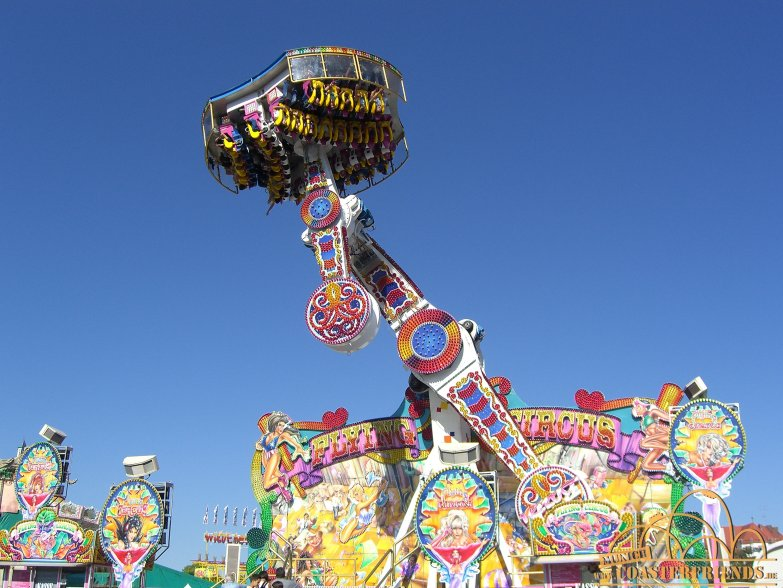
\includegraphics[width=.7\textwidth]{images/fig_00}

%\textit{Centrifugeuse humaine développée par le CNRS / MEDES } 

}%figues de la page de garde

\def\xxpied{%
Révision cinématique -- Modélisation cinématique\\
Fiche 2 -- \xxactivite%
}

\setcounter{secnumdepth}{5}
%---------------------------------------------------------------------------


%%UTF8
%% macros-mecanique version 26-mai-2013
%\usepackage[francais, frenchb]{babel}
%\usepackage[T1]{fontenc}
%\usepackage[utf8]{inputenc}
%\usepackage{url}
%\usepackage{multicol}
%\usepackage{graphicx}
%\usepackage{xargs}
%%\usepackage[usenames,svgnames,dvipsnames]{xcolor}  %pas pour AMC
%\usepackage[leqno, fleqn]{amsmath}
%\usepackage{amssymb}
%\usepackage{mathtools}
%\usepackage{wrapfig}
%\usepackage{enumerate}
%\usepackage{longtable}
%\usepackage{tabularx}
\usepackage{tikz}
%\usetikzlibrary{shapes}
%\usetikzlibrary{calc}
%\usepackage{enumitem}
%\usepackage{fancyhdr}
%\usepackage{caption}
%\usepackage{subcaption}
%\usepackage{ifthen}
%\usepackage{calc}
%\usepackage{fp}
%\usepackage{multido}
%\usepackage{lscape}
%\usepackage{titling}
%\usepackage{cancel}
%\usepackage{geometry}
%\usepackage{float}
%%\usepackage{palatino}  %pas pour AMC
%\usepackage{hyperref}
%\usepackage{subscript}
%\usepackage{movie15}
%\usepackage{siunitx}  %pas pour AMC
%\usepackage{auto-greek}
%\usepackage{floatfig}




% Xavier
%\usepackage[adobe-utopia]{mathdesign}
%\usepackage{framed}
%\usepackage[normalem]{ulem}
%\usepackage{titlesec}
%\usepackage{vmargin}
%\usepackage{longtable}
%\usepackage{subfig}
%\usepackage{color}
%\usepackage{colortbl}
%
%
\definecolor{gris25}{gray}{0.75}
\definecolor{gris15}{gray}{0.85}
%\definecolor{bleu}{RGB}{18,33,98}
%\definecolor{bleuf}{RGB}{42,94,171}
%\definecolor{bleuc}{RGB}{231,239,247}
%\definecolor{rougef}{RGB}{185,18,27}
%\definecolor{rougec}{RGB}{255,230,231}
%\definecolor{vertf}{RGB}{103,126,82}
%\definecolor{vertc}{RGB}{220,255,191}
%

%Symbole degres \deg
\renewcommand{\deg}{\ensuremath{^\circ}\xspace}

%norme d'un vecteur
\newcommand{\norme}[1]{\ensuremath{\|#1 \|}}
%grande fleche sur les vecteurs : \gv
\newcommand{\gv}[1]{\ensuremath{\overrightarrow{#1}}}
%%vecteurs de base raccourcis
%\newcommand{\vx}[1]{\ensuremath{\vec{x}_{#1}}}
%\newcommand{\vy}[1]{\ensuremath{\vec{y}_{#1}}}
%\newcommand{\vz}[1]{\ensuremath{\vec{z}_{#1}}}

%coordonnees de vecteurs		  			
\newcommand{\coordvecteur}[3]{\begin{pmatrix} #1 \\ #2\\ #3 \end{pmatrix}}   
% pour les torseurs
%indice en bas a gauche (torseurs) \indicegauche
\newcommand{\indicegauche}[2]{{\vphantom{#2}}_{#1}#2}
% nom d'un torseur d'action meca \nomtorseur
\newcommand{\nomtorseur}[2]{\left\{ \mathcal{#1}_{#2} \right\}}

%Torseur d'action mécanique
\newcommand{\torseuram}[2]{\ensuremath{\left\{ \mathcal{T}_{#1 \to #2} \right\}}}


% torseur sous la forme développée en coordonnees pluckeriennes
\newcommand{\coordtorseur}[7]{\ensuremath{\indicegauche{#1}{\begin{Bmatrix} #2 & #5 \\ #3 & #6 \\ #4 & #7 \end{Bmatrix}}}}
% torseur phantom
\newcommand{\torseurphantom}{\ensuremath{\vphantom{\indicegauche{0}{\begin{Bmatrix} 0 & 0 \\ 0 & 0 \\ 0 & 0 \end{Bmatrix}}}}}
\newcommand{\composanteOmegaTorseur}[3]{\omega_{#1_{#2#3}}}
\newcommand{\composanteVitesseTorseur}[3]{v_{#1_{#2#3}}}
% torseur sous la forme developpee en coordonnees pluckeriennes avec base xyz
\newcommand{\coordtorseurxyz}[7]{\ensuremath{\indicegauche{#1}{\begin{Bmatrix} #2 & #5 \\ #3 & #6 \\ #4 & #7 \end{Bmatrix}_{(\vec{x},\vec{y},\vec{z})}}}}
\newcommand{\torcindev}[9]{
\coordtorseur{#1}{\ifthenelse{#2=1}{\composanteOmegaTorseur{x}{#8}{#9}}{0}}{\ifthenelse{#3=1}{\composanteOmegaTorseur{y}{#8}{#9}}{0}}{\ifthenelse{#4=1}{\composanteOmegaTorseur{z}{#8}{#9}}{0}}{\ifthenelse{#5=1}{\composanteVitesseTorseur{x}{#8}{#9}}{0}}{\ifthenelse{#6=1}{\composanteVitesseTorseur{y}{#8}{#9}}{0}}{\ifthenelse{#7=1}{\composanteVitesseTorseur{z}{#8}{#9}}{0}}
}
% d droit pour la differentielle
\newcommand{\dd}{\mathrm{d}}
%vecteur vitesse
\newcommand{\vecvit}[3]{\ensuremath{\gv{V}_{#1\in #2 / #3}}}
%vecteur taux de rotation
\newcommand{\vecrot}[2]{\ensuremath{\gv{\Omega}_{#1 / #2}}}
%vecteur acceleration
\newcommand{\vecacc}[3]{\ensuremath{\gv{\Gamma}_{#1 \in #2 / #3}}}
% vecteur force
\newcommand{\vecforce}[3]{\ensuremath{\gv{#1}_{#2 \to #3}}}
% vecteur moment
\newcommand{\vecmoment}[2]{\ensuremath{\gv{M}_{#1(#2)}}}
% Mouvement
\newcommand{\mvt}[2]{\ensuremath{\text{Mvt}_{#1 / #2}}}
% Torseur cinematique
\newcommand{\torcin}[2]{\ensuremath{\left\{ \mathcal{V}_{#1 / #2} \right\}}}
% derivee d'un vecteur par rapport au temps, et dans un referentiel donne
\newcommand{\derivect}[2]{\ensuremath{\left( \frac{\dd #1}{\dd t} \right)_{#2}}}
% dérivée d'un vecteur par rapport au temps, et dans un référentiel donné, grande fraction (texte)
\newcommand{\gderivect}[2]{\ensuremath{\left( \dfrac{\dd #1}{\dd t} \right)_{#2}}}
% forme littérale d'un torseur
\newcommand{\torlit}[3]{{\indicegauche{#1}{\begin{Bmatrix} #2 \\ #3  \end{Bmatrix}}}}
% Trajectoire d'un point
\newcommand{\traj}[3]{\ensuremath{T_{#1 \in #2/#3}}}
% derivee scalaire par rapport au temps
\newcommand{\derit}[1]{\frac{\mathrm{d}#1}{\mathrm{d}t}}
% différentielle droite \ud
%\newcommand{\ud}{\mathrm{d}}
% calcul d'un produit vectoriel par les composantes (entiers relatifs uniquement)
\newcommand{\prodvec}[6]{\ensuremath{
\FPeval\respvx{trunc(((#2*#6)-(#3*#5)),0)}
\FPeval\respvy{trunc(((#3*#4)-(#1*#6)),0)}
\FPeval\respvz{trunc(((#1*#5)-(#2*#4)),0)}
\begin{pmatrix}
 \respvx \\
 \respvy \\
 \respvz 
\end{pmatrix}
}}
% systeme d'equations
\newcommand{\systeq}[1]{\ensuremath{\left\{ \begin{aligned} #1 \end{aligned}\right.}}

%pour générer des copies à trous
\newcommand{\acompleter}[1]{\ifthenelse{\boolean{version-a-trous}}{\phantom{{\Large{#1\xspace}}}}{\textcolor{red}{#1}}}

% mise en forme
% exemple
%\newcommand{\exemple}[1]{\paragraph{Exemple :} #1}
% exemple
\newcommand{\exemples}[1]{\paragraph{Exemples :} #1}



% pour encadrer dans un alignement
\makeatletter
\newlength{\boxed@align@width}
\newcommand{\boxedalign}[2]{
#1 & \setlength{\boxed@align@width}{\widthof{$\displaystyle#1$}+1.4pt+1.4pt}
\hspace{-\boxed@align@width}\boxed{\vphantom{#1}\hspace{\boxed@align@width}#2}}
\makeatother
%%%%

%%%%%%%%%%%%%%%%%%%%%%%%%%%%%%%%%

%Commande pour tracer des figures planes: \figureplane
\newcommand\figureplane[9]{
\begin{tikzpicture}[scale=#9]
\draw[thick,->,#7] (0,0) -- (0:1) node[anchor=north west]{$\vec{#1}$};
\draw[thick,->,#7] (0,0) -- (90:1) node[anchor=north east]{$\vec{#3}$}; 
\draw[thick,->,#8] (0,0) -- (20:1) node[anchor=south east]{$\vec{#2}$}; 
\draw[thick,->,#8] (0,0) -- (110:1) node[anchor=north east]{$\vec{#4}$}; 
\fill[white] (0,0) circle (0.05);
\draw[thick,#7] (0,0) circle (0.05);
\fill[#7] (0,0) circle (0.01);
\draw (-0.05,0) node[anchor=north east] {$\vec{#5}$};
\draw[thick,->] (0.4,0) arc (0:20:0.4);
\draw[thick,->] (0,0.4) arc (90:110:0.4);
\draw (0.4,0.08) node[anchor=west] {$#6$};
\draw (-0.08,0.4) node[anchor=south] {$#6$};
\end{tikzpicture}
}

%couleurs des figures planes pour ne pas dépasser neuf arguments
\newcommand\couleursfigureplane[2]{%
    \def\premierecouleur{#1}%
    \def\deuxiemecouleur{#2}%
}


%Commande pour tracer des figures planes avec reperes: \figureplanerep
\newcommand\figureplanerep[9]{
\begin{tikzpicture}[scale=#9]
\draw[thick,->,\premierecouleur ] (0,0) -- (0:1) node[anchor=north west]{$\vec{#1}$};
\draw[thick,->,\premierecouleur ] (0,0) -- (90:1) node[anchor=north east]{$\vec{#3}$}; 
\draw[thick,->,\deuxiemecouleur ] (0,0) -- (20:1) node[anchor=south east]{$\vec{#2}$}; 
\draw[thick,->,\deuxiemecouleur ] (0,0) -- (110:1) node[anchor=north east]{$\vec{#4}$}; 
\fill[white] (0,0) circle (0.05);
\draw[thick,\premierecouleur] (0,0) circle (0.05);
\fill[\premierecouleur] (0,0) circle (0.01);
\draw[\premierecouleur] (-0.05,0) node[anchor=north east] {$\vec{#5}$};
\draw[thick,->] (0.4,0) arc (0:20:0.4);
\draw[thick,->] (0,0.4) arc (90:110:0.4);
\draw[thick,\premierecouleur] (0:0.5) arc (180:360:0.15) ;
\draw[\premierecouleur] (0.65,-0.07) node{\ensuremath{#7}};
\draw[thick,\deuxiemecouleur] (20:0.8) arc (20:200:0.15);
\draw[\deuxiemecouleur] (0.59,0.29) node{\ensuremath{#8}};
\draw (0.4,0.08) node[anchor=west] {$#6$};
\draw (-0.08,0.4) node[anchor=south] {$#6$};
\end{tikzpicture}
}

%Commande pour tracer des figures planes autour de z avec reperes: \figureplanerepz
\newcommand\figureplanerepz[9]{
\begin{tikzpicture}[scale=#9]
\draw[thick,->, #7] (0,0) -- (0:1) node[anchor=north west]{$\vec{x}_{#1}$};
\draw[thick,->, #7] (0,0) -- (90:1) node[anchor=north east]{$\vec{y}_{#1}$}; 
\draw[thick,->, #8] (0,0) -- (20:1) node[anchor=south east]{$\vec{x}_{#2}$}; 
\draw[thick,->, #8] (0,0) -- (110:1) node[anchor=north east]{$\vec{y}_{#2}$}; 
\fill[white] (0,0) circle (0.05);
\draw[thick, #7] (0,0) circle (0.05);
\fill[#7] (0,0) circle (0.01);
\draw[#7] (-0.05,0) node[anchor=north east] {$\vec{z}_{#3}$};
\draw[thick,->] (0.4,0) arc (0:20:0.4);
\draw[thick,->] (0,0.4) arc (90:110:0.4);
\draw (0.4,0.08) node[anchor=west] {$#4$};
\draw (-0.08,0.4) node[anchor=south] {$#4$};
\draw[#7] [thick] (0:0.5) arc (180:360:0.15) ;
\draw[#7] (0.65,-0.07) node{\ensuremath{#5}};
\draw[#8] [thick] (20:0.8) arc (20:200:0.15);
\draw[#8] (0.59,0.29) node{\ensuremath{#6}};
\end{tikzpicture}
}

%Commande pour tracer des figures planes autour de x avec reperes: \figureplanerepx
\newcommand\figureplanerepx[9]{
\begin{tikzpicture}[scale=#9]
\draw[thick,->, #7] (0,0) -- (0:1) node[anchor=north west]{$\vec{y}_{#1}$};
\draw[thick,->, #7] (0,0) -- (90:1) node[anchor=north east]{$\vec{z}_{#1}$}; 
\draw[thick,->, #8] (0,0) -- (20:1) node[anchor=south east]{$\vec{y}_{#2}$}; 
\draw[thick,->, #8] (0,0) -- (110:1) node[anchor=north east]{$\vec{z}_{#2}$}; 
\fill[white] (0,0) circle (0.05);
\draw[thick, #7] (0,0) circle (0.05);
\fill[#7] (0,0) circle (0.01);
\draw[#7] (-0.05,0) node[anchor=north east] {$\vec{x}_{#3}$};
\draw[thick,->] (0.4,0) arc (0:20:0.4);
\draw[thick,->] (0,0.4) arc (90:110:0.4);
\draw (0.4,0.08) node[anchor=west] {$#4$};
\draw (-0.08,0.4) node[anchor=south] {$#4$};
\draw[#7] [thick] (0:0.5) arc (180:360:0.15) ;
\draw[#7] (0.65,-0.07) node{\ensuremath{#5}};
\draw[#8] [thick] (20:0.8) arc (20:200:0.15);
\draw[#8] (0.59,0.29) node{\ensuremath{#6}};
\end{tikzpicture}
}

%Commande pour tracer des figures planes autour de y avec reperes: \figureplanerepy
\newcommand\figureplanerepy[9]{
\begin{tikzpicture}[scale=#9]
\draw[thick,->, #7] (0,0) -- (0:1) node[anchor=north west]{$\vec{z}_{#1}$};
\draw[thick,->, #7] (0,0) -- (90:1) node[anchor=north east]{$\vec{x}_{#1}$}; 
\draw[thick,->, #8] (0,0) -- (20:1) node[anchor=south east]{$\vec{z}_{#2}$}; 
\draw[thick,->, #8] (0,0) -- (110:1) node[anchor=north east]{$\vec{x}_{#2}$}; 
\fill[white] (0,0) circle (0.05);
\draw[thick, #7] (0,0) circle (0.05);
\fill[#7] (0,0) circle (0.01);
\draw[#7] (-0.05,0) node[anchor=north east] {$\vec{y}_{#3}$};
\draw[thick,->] (0.4,0) arc (0:20:0.4);
\draw[thick,->] (0,0.4) arc (90:110:0.4);
\draw (0.4,0.08) node[anchor=west] {$#4$};
\draw (-0.08,0.4) node[anchor=south] {$#4$};
\draw[#7] [thick] (0:0.5) arc (180:360:0.15) ;
\draw[#7] (0.65,-0.07) node{\ensuremath{#5}};
\draw[#8] [thick] (20:0.8) arc (20:200:0.15);
\draw[#8] (0.59,0.29) node{\ensuremath{#6}};
\end{tikzpicture}
}

%%% Graphe des liaisons%%%%%%%%%%%%

%\begin{tikzpicture}[scale=1]
%\tikzstyle{sommet}=[draw,ellipse,minimum height=1.5cm,fill=gray!20]
%\tikzstyle{liaison}=[text width=2cm, text centered]
%\node[sommet] (0) at (360/3*0:3) {Bâti 0};
%\node[sommet] (1) at (360/3*1:3) {Coulisseau 1};
%\node[sommet] (2) at (360/3*2:3) {Panneau 2};
%\draw (1) to[bend right=20] (2);
%\draw (2) to[bend right=20] (0);
%\draw (0) to[bend right=20] (1);
%\node[liaison] at (360/3*0.4:3.2) {Glissière de direction \vx{0}} ;
%\node[liaison] at (360/3*1.5:3.2) {Ponctuelle de normale $(B,\vx{2})$} ;
%\node[liaison] at (360/3*2.6:3.3) {Pivot d'axe $(C,\vz{0})$} ;
%\end{tikzpicture}

%Commande pour tracer des bases isometriques: \baseiso
\newcommand\baseiso[5]{
\begin{tikzpicture}[scale=#5*0.82]
\draw[->] (0,0) -- (-30:1) node[anchor=north west]{$\vec{#1}$};
\draw[->] (0,0) -- (90:1) node[anchor=east]{$\vec{#2}$}; 
\draw[->] (0,0) -- (210:1) node[anchor=north east]{$\vec{#3}$};
\draw node[anchor=south east]{#4};
\end{tikzpicture}
}


%Commande pour tracer des bases planes: \baseplane
\newcommand\baseplane[4]{
\begin{tikzpicture}[scale=#4]
\draw[->] (0,0) -- (0:1) node[anchor=north west]{$\vec{#1}$};
\draw[->] (0,0) -- (90:1) node[anchor=south east]{$\vec{#2}$}; 
\draw node[anchor=north east]{#3};
\end{tikzpicture}
}

%Commande pour tracer des bases en 2D avec vecteur sortant, tournées d'un certain angle : \basevecteursortant
\newcommand\basevecteursortant[5]{
\begin{tikzpicture}[scale=#5]
\draw[->] (0,0) -- (0+#4:1) node[anchor=north west]{$\vec{#1}$};
\draw[->] (0,0) -- (90+#4:1) node[anchor=south east]{$\vec{#2}$}; 
\fill[white] (0,0) circle (0.05);
\draw[thick] (0,0) circle (0.05);
\fill (0,0) circle (0.01);
\draw (-0.05,0) node[anchor=north east] {$\vec{#3}$};
\end{tikzpicture}
}

%Commande pour tracer des bases en 2D avec vecteur rentrant, tournées d'un certain angle : \basevecteurrentrant
\newcommand\basevecteurrentrant[5]{
\begin{tikzpicture}[scale=#5]
\draw[->] (0,0) -- (#4:1) node[anchor=north west]{$\vec{#1}$};
\draw[->] (0,0) -- (90+#4:1) node[anchor=south east]{$\vec{#2}$}; 
\fill[white] (0,0) circle (0.05);
\draw[thick] (0,0) circle (0.05);
\draw (225:0.05) -- (45:0.05);
\draw (135:0.05) -- (-45:0.05);
\draw (-0.05,0) node[anchor=north east] {$\vec{#3}$};
\end{tikzpicture}
}

%Commande pour tracer des bases planes tournées d'un certain angle: \baseplanerot
\newcommand\baseplanerot[5]{
\begin{tikzpicture}[scale=#5]
\draw[->] (0,0) -- (0+#4:1) node[anchor=north west]{$\vec{#1}$};
\draw[->] (0,0) -- (90+#4:1) node[anchor=south east]{$\vec{#2}$}; 
\draw node[anchor=north east]{#3};
\end{tikzpicture}
}

%Commande pour tracer des tableaux de ddl : tabddl
\newcommand\tabddl[6]{
\begin{tabular}{|c|c|}
\hline 
\ensuremath{#1} & \ensuremath{#4} \\ 
\hline 
\ensuremath{#2} & \ensuremath{#5} \\ 
\hline 
\ensuremath{#3} & \ensuremath{#6} \\ 
\hline 
\end{tabular} 
}

%Commande pour tracer des tableaux de ddl vides : tabddlvide
\newcommand\tabddlvide{
\begin{tabular}{|c|c|}
\hline 
$\phantom{T_x}$ & $\phantom{T_x}$ \\ 
\hline 
$\phantom{T_x}$ & $\phantom{T_x}$ \\ 
\hline 
$\phantom{T_x}$ & $\phantom{T_x}$ \\ 
\hline 
\end{tabular} 
}


%%% figure pour projeter un vecteur avec un angle quelconque \figureprojection{x}{y}{z}{u}{v}{\theta}{40}{4}
\newcommand\figureprojection[8]{
\begin{tikzpicture}[scale=#8]
\draw[thick,->] (0,0) -- (0:1); 
\draw (0:1.1) node {$\vec{#1}$};
\draw[thick,->] (0,0) -- (90:1);
\draw (90:1.1) node {$\vec{#2}$}; 
\draw[thick,->] (0,0) -- (#7:1);
\draw (#7:1.1) node {$\vec{#4}$}; 
\draw[thick,->] (0,0) -- (90+#7:1);
\draw (90+#7:1.1) node {$\vec{#5}$}; 
\fill[white] (0,0) circle (0.05);
\draw[thick] (0,0) circle (0.05);
\fill (0,0) circle (0.01);
\draw (-0.05,0) node[anchor=north east] {$\vec{#3}$};
\draw[thick,->] (0.4,0) arc (0:#7:0.4);
\draw[thick,->] (0,0.4) arc (90:90+#7:0.4);
\draw (#7/2:0.5) node {$#6$};
\draw (#7/2+90:0.5) node {$#6$};
\end{tikzpicture}
}

\newcommand\laplace[1]{L(#1)}

\newcommand\baseisoxyz{\baseiso{x}{y}{z}{A}{2}}
\newcommand\baseplanexy{\baseplane{x}{y}{A}{2}}
\newcommand\baseplaneyz{\baseplane{y}{z}{A}{2}}
\newcommand\baseplanezx{\baseplane{z}{x}{A}{2}}
\begin{document}
%\chapterimage{images/Fond_Cin}
\pagestyle{empty}


%%%%%%%% PAGE DE GARDE COURS
\ifcours
% ==== BANDEAU DES TITRES ==== 
\begin{tikzpicture}[remember picture,overlay]
\node at (current page.north west)
{\begin{tikzpicture}[remember picture,overlay]
\node[anchor=north west,inner sep=0pt] at (0,0) {\includegraphics[width=\paperwidth]{\thechapterimage}};
\draw[anchor=west] (-2cm,-8cm) node [line width=2pt,rounded corners=15pt,draw=ocre,fill=white,fill opacity=0.6,inner sep=40pt]{\strut\makebox[22cm]{}};
\draw[anchor=west] (1cm,-8cm) node {\huge\sffamily\bfseries\color{black} %
\begin{minipage}{1cm}
\rotatebox{90}{\LARGE\sffamily\textsc{\color{ocre}\textbf{\xxnumpartie}}}
\end{minipage} \hfill
\begin{minipage}[c]{14cm}
\begin{titrepartie}
\begin{flushright}
\renewcommand{\baselinestretch}{1.1} 
\Large\sffamily\textsc{\textbf{\xxpartie}}
\renewcommand{\baselinestretch}{1} 
\end{flushright}
\end{titrepartie}
\end{minipage} \hfill
\begin{minipage}[c]{3.5cm}
{\large\sffamily\textsc{\textbf{\color{ocre} \discipline}}}
\end{minipage} 
 };
\end{tikzpicture}};
\end{tikzpicture}
% ==== FIN BANDEAU DES TITRES ==== 


% ==== ONGLET 
\begin{tikzpicture}[overlay]
\node[shape=rectangle, 
      rounded corners = .25 cm,
	  draw= ocre,
	  line width=2pt, 
	  fill = ocre!10,
	  minimum width  = 2.5cm,
	  minimum height = 3cm,] at (18.3cm,0) {};
\node at (17.7cm,0) {\rotatebox{90}{\textbf{\Large\color{ocre}{\classe}}}};
%{};
\end{tikzpicture}
% ==== FIN ONGLET 


\vspace{3.5cm}

\begin{tikzpicture}[remember picture,overlay]
\draw[anchor=west] (-2cm,-6cm) node {\huge\sffamily\bfseries\color{black} %
\begin{minipage}{2cm}
\begin{center}
\LARGE\sffamily\textsc{\color{ocre}\textbf{\xxactivite}}
\end{center}
\end{minipage} \hfill
\begin{minipage}[c]{15cm}
\begin{titrechapitre}
\renewcommand{\baselinestretch}{1.1} 
\Large\sffamily\textsc{\textbf{\xxnumchapitre}}

\Large\sffamily\textsc{\textbf{\xxchapitre}}
\vspace{.5cm}

\renewcommand{\baselinestretch}{1} 
\normalsize\normalfont
\xxcompetences
\end{titrechapitre}
\end{minipage}  };
\end{tikzpicture}
\vfill

\begin{flushright}
\begin{minipage}[c]{.3\linewidth}
\begin{center}
\xxfigures
\end{center}
\end{minipage}\hfill
\begin{minipage}[c]{.6\linewidth}
\startcontents
%\printcontents{}{1}{}
\printcontents{}{1}{}
\end{minipage}
\end{flushright}

\begin{tikzpicture}[remember picture,overlay]
\draw[anchor=west] (4.5cm,-.7cm) node {
\begin{minipage}[c]{.2\linewidth}
\begin{flushright}

\includegraphics[width=2cm]{logoCC}
\end{flushright}
\end{minipage}
\begin{minipage}[c]{.2\linewidth}
\textsl{\xxauteur} \\
\textsl{\classe}
\end{minipage}
 };
\end{tikzpicture}

\newpage
\pagestyle{fancy}

%\newpage
%\pagestyle{fancy}

\else
\fi
%% FIN PAGE DE GARDE DES COURS

%%%%%%%% PAGE DE GARDE TD
\iftd
%\begin{tikzpicture}[remember picture,overlay]
%\node at (current page.north west)
%{\begin{tikzpicture}[remember picture,overlay]
%\draw[anchor=west] (-2cm,-3.25cm) node [line width=2pt,rounded corners=15pt,draw=ocre,fill=white,fill opacity=0.6,inner sep=40pt]{\strut\makebox[22cm]{}};
%\draw[anchor=west] (1cm,-3.25cm) node {\huge\sffamily\bfseries\color{black} %
%\begin{minipage}{1cm}
%\rotatebox{90}{\LARGE\sffamily\textsc{\color{ocre}\textbf{\xxnumpartie}}}
%\end{minipage} \hfill
%\begin{minipage}[c]{13.5cm}
%\begin{titrepartie}
%\begin{flushright}
%\renewcommand{\baselinestretch}{1.1} 
%\Large\sffamily\textsc{\textbf{\xxpartie}}
%\renewcommand{\baselinestretch}{1} 
%\end{flushright}
%\end{titrepartie}
%\end{minipage} \hfill
%\begin{minipage}[c]{3.5cm}
%{\large\sffamily\textsc{\textbf{\color{ocre} \discipline}}}
%\end{minipage} 
% };
%\end{tikzpicture}};
%\end{tikzpicture}

%%%%%%%%%% PAGE DE GARDE TD %%%%%%%%%%%%%%%
%\begin{tikzpicture}[overlay]
%\node[shape=rectangle, 
%      rounded corners = .25 cm,
%	  draw= ocre,
%	  line width=2pt, 
%	  fill = ocre!10,
%	  minimum width  = 2.5cm,
%	  minimum height = 2.5cm,] at (18.5cm,0) {};
%\node at (17.7cm,0) {\rotatebox{90}{\textbf{\Large\color{ocre}{\classe}}}};
%%{};
%\end{tikzpicture}

% PARTIE ET CHAPITRE
%\begin{tikzpicture}[remember picture,overlay]
%\draw[anchor=west] (-1cm,-2.1cm) node {\large\sffamily\bfseries\color{black} %
%\begin{minipage}[c]{15cm}
%\begin{flushleft}
%\xxnumchapitre \\
%\xxchapitre
%\end{flushleft}
%\end{minipage}  };
%\end{tikzpicture}

% BANDEAU EXO
\iflivret % SI LIVRET
\begin{tikzpicture}[remember picture,overlay]
\draw[anchor=west] (-2cm,-3.3cm) node {\huge\sffamily\bfseries\color{black} %
\begin{minipage}{5cm}
\begin{center}
\LARGE\sffamily\color{ocre}\textbf{\textsc{\xxactivite}}

\begin{center}
\xxfigures
\end{center}

\end{center}
\end{minipage} \hfill
\begin{minipage}[c]{12cm}
\begin{titrechapitre}
\renewcommand{\baselinestretch}{1.1} 
\large\sffamily\textbf{\textsc{\xxtitreexo}}

\small\sffamily{\textbf{\textit{\color{black!70}\xxsourceexo}}}
\vspace{.5cm}

\renewcommand{\baselinestretch}{1} 
\normalsize\normalfont
\xxcompetences
\end{titrechapitre}
\end{minipage}};
\end{tikzpicture}
\else % ELSE NOT LIVRET
\begin{tikzpicture}[remember picture,overlay]
\draw[anchor=west] (-2cm,-4.5cm) node {\huge\sffamily\bfseries\color{black} %
\begin{minipage}{5cm}
\begin{center}
\LARGE\sffamily\color{ocre}\textbf{\textsc{\xxactivite}}

\begin{center}
\xxfigures
\end{center}

\end{center}
\end{minipage} \hfill
\begin{minipage}[c]{12cm}
\begin{titrechapitre}
\renewcommand{\baselinestretch}{1.1} 
\large\sffamily\textbf{\textsc{\xxtitreexo}}

\small\sffamily{\textbf{\textit{\color{black!70}\xxsourceexo}}}
\vspace{.5cm}

\renewcommand{\baselinestretch}{1} 
\normalsize\normalfont
\xxcompetences
\end{titrechapitre}
\end{minipage}};
\end{tikzpicture}

\fi

\else   % FIN IF TD
\fi


%%%%%%%% PAGE DE GARDE FICHE
\iffiche
\begin{tikzpicture}[remember picture,overlay]
\node at (current page.north west)
{\begin{tikzpicture}[remember picture,overlay]
\draw[anchor=west] (-2cm,-2.25cm) node [line width=2pt,rounded corners=15pt,draw=ocre,fill=white,fill opacity=0.6,inner sep=40pt]{\strut\makebox[22cm]{}};
\draw[anchor=west] (1cm,-2.25cm) node {\huge\sffamily\bfseries\color{black} %
\begin{minipage}{1cm}
\rotatebox{90}{\LARGE\sffamily\textsc{\color{ocre}\textbf{\xxnumpartie}}}
\end{minipage} \hfill
\begin{minipage}[c]{14cm}
\begin{titrepartie}
\begin{flushright}
\renewcommand{\baselinestretch}{1.1} 
\large\sffamily\textsc{\textbf{\xxpartie} \\} 

\vspace{.2cm}

\normalsize\sffamily\textsc{\textbf{\xxnumchapitre -- \xxchapitre}}
\renewcommand{\baselinestretch}{1} 
\end{flushright}
\end{titrepartie}
\end{minipage} \hfill
\begin{minipage}[c]{3.5cm}
{\large\sffamily\textsc{\textbf{\color{ocre} \discipline}}}
\end{minipage} 
 };
\end{tikzpicture}};
\end{tikzpicture}

\iflivret
\begin{tikzpicture}[overlay]
\node[shape=rectangle, 
      rounded corners = .25 cm,
	  draw= ocre,
	  line width=2pt, 
	  fill = ocre!10,
	  minimum width  = 2.5cm,
	  minimum height = 2.5cm,] at (18.5cm,.5cm) {};
\node at (17.9cm,.5cm) {\rotatebox{90}{\textsf{\textbf{\large\color{ocre}{\classe}}}}};
%{};
\end{tikzpicture}
\else
\begin{tikzpicture}[overlay]
\node[shape=rectangle, 
      rounded corners = .25 cm,
	  draw= ocre,
	  line width=2pt, 
	  fill = ocre!10,
	  minimum width  = 2.5cm,
%	  minimum height = 2.5cm,] at (18.5cm,1.1cm) {};
	  minimum height = 2.5cm,] at (18.6cm,0.5cm) {};
\node at (18cm,0.5cm) {\rotatebox{90}{\textsf{\textbf{\large\color{ocre}{\classe}}}}};
%{};
\end{tikzpicture}

\fi

\else
\fi



\vspace{5cm}
\pagestyle{fancy}
\thispagestyle{plain}


\def\columnseprulecolor{\color{ocre}}
\setlength{\columnseprule}{0.4pt} 

\ifprof
\else
\begin{multicols}{2}
\fi


La manège Magic Arms dont la modélisation ainsi qu'un extrait de cahier des charges fonctionnel est composé d'une structure métallique d'environ \SI{12}{m} de haut avec deux bras mobiles. Les passagers s'assoient sur 39 pièces disposées sur une plate-forme tournante. Dès que tous les passagers sont assis et attachés, la nacelle tourne autour de son axe, le bras principal (bras \textbf{1}) et le bras secondaires (bras \textbf{2}), liés l'un à l'autre au début du cycle, commencent à tourner. Après 9 secondes, le maximum de hauteur est atteint et les deux bras se désindexent et se mettent à tourner indépendamment l'un de l'autre. Tous les mouvements sont pilotés par ordinateur. 

\begin{center}
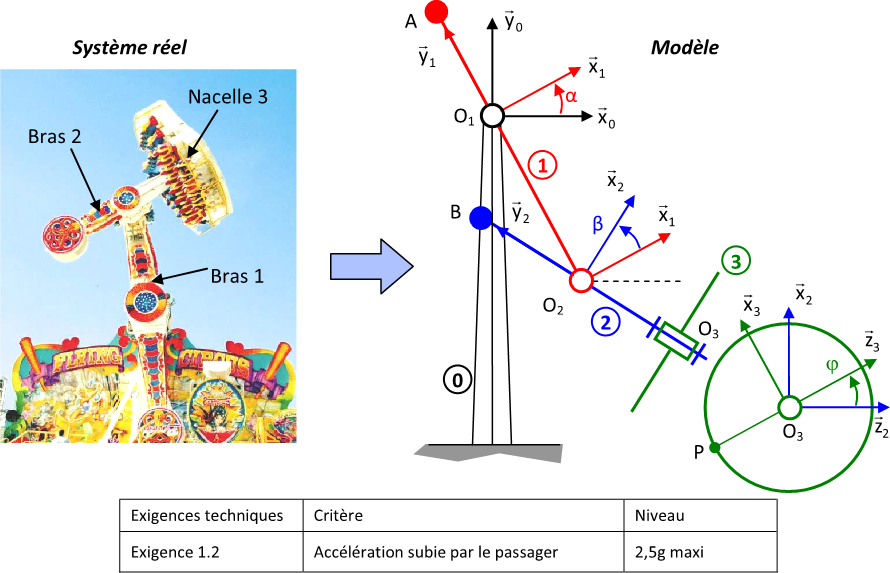
\includegraphics[width=\linewidth]{images/img1}
\end{center}

Le manège, schématisé ci-dessus, comporte :
\begin{itemize}
\item un bras principal \textbf{1} assimilé à une barre $AO_1O_2$. Il est en liaison pivot parfait d'axe $(O_1,\vect{z_1})$ caractérisée par le paramètre $\alpha$ avec le bâti \textbf{0}. On pose $\vect{O_1O_2}=-l_1\vect{y_1}$;
\item un bras secondaire 2 assimilé à une barre $BO_2O_3$. Il est en liaison pivot parfait d'axe $(O_2,\vect{z_2})$ caractérisée par le paramètre $\beta$ avec le bras principal \textbf{1}. On pose $\vect{O_2O_3}=-l_2\vect{y_2}$;
\item une nacelle \textbf{2} assimilée à un disque de centre $O_3$ et de rayon $R$. Elle est en liaison parfaite d'axe $(O_3,\vect{y_2})$ caractérisée par le paramètre $\varphi$ avec le bras \textbf{2}. On s'intéresse plus particulièrement à un passager considéré comme un point matériel $P$ tel que $\vect{O_3P}=-R\vect{z_3}$.
\end{itemize}
\subparagraph{}
\textit{Construire les figures planes associées au schéma cinématique.}
\ifprof

\begin{corrige}
\couleursfigureplane{black}{red}
\figureplanerep{x_0}{x_1}{y_0}{y_1}{z_0}{\alpha}{0}{1}{3}
\couleursfigureplane{red}{blue}
\figureplanerep{x_1}{x_2}{y_1}{y_2}{z_0}{\beta}{1}{2}{3}
\couleursfigureplane{blue}{green}
\figureplanerep{z_0}{z_3}{x_2}{x_3}{y_2}{\varphi}{2}{3}{3}

\end{corrige}\else\fi

\subparagraph{}
\textit{Calculer $\vecto{1}{0}$, $\vecto{2}{1}$ et $\vecto{3}{2}$.}
\ifprof
\begin{corrige}
\begin{align*}
\vecrot{1}{0}&=\dot\alpha\vect{z_0}\\
\vecrot{2}{1}&=\dot\beta\vect{z_0}\\
\vecrot{3}{2}&=\dot\varphi\vect{y_2}\\
\end{align*}
\end{corrige}\else\fi

%\vspace{.3cm}

%On admet que $\vecto{3}{0}=\vecto{3}{2}+\vecto{2}{1}+\vecto{1}{0}$.

\subparagraph{}
\textit{Calculer $\vecto{2}{0}$ et $\vecto{3}{0}$.}
\ifprof
\begin{corrige}
\begin{align*}
\vecrot{2}{0}&=\vecrot{2}{1}+\vecrot{1}{0}\\
	&=(\dot\alpha+\dot\beta)\vect{z_0}\\
\vecrot{3}{0}&=\vecrot{3}{2}+\vecrot{2}{0}\\
	&=(\dot\alpha+\dot\beta)\vect{z_0}+\dot\varphi\vect{y_2}
\end{align*}

\end{corrige}\else\fi

\subparagraph{}
\textit{Calculer les produits vectoriels suivants : $\vect{z_2}\wedge\vect{z_3}$,
$\vect{x_3}\wedge\vect{x_2}$, $\vect{x_3}\wedge\vect{z_2}$,
$\vect{z_2}\wedge\vect{z_1}$, $\vect{x_2}\wedge\vect{x_0}$,
$\vect{x_3}\wedge\vect{z_0}$.}
\ifprof
\begin{corrige}

\begin{align*}
\vect{z_2} \wedge \vect{z_3} &=\sin\varphi \vect{y_2}\\
\vect{x_3} \wedge\vect{x_2} &= -\sin\varphi \vect{y_2}\\
\vect{x_3} \wedge \vect{z_2}&= -\sin\left(\dfrac{\pi}{2}+\varphi\right)\vect{y_2}\\
	&=-\cos\varphi\vect{y_2}\\
\vect{z_2} \wedge \vz1 &= \vec{0}\\
\vect{x_2} \wedge \vx0 &= \left(\cos\beta\vx1+\sin\beta\vy1\right)\wedge\vx0\\
	&=-\cos\beta\sin\alpha\vect{z_0} - \sin\beta\sin\left(\dfrac{\pi}{2}+\alpha\right)\vect{z_0}\\
	&=(-\cos\beta\sin\alpha-\sin\beta\cos\alpha)\vect{z_0}\\
	&=-\sin(\beta+\alpha)\vect{z_0}\\
\vect{x_3}\wedge\vect{z_0} &= -\sin\left(\dfrac{\pi}{2}+\varphi\right)\vect{y_2}\\
	&=-\cos\varphi\vect{y_2}
\end{align*}

\end{corrige}\else\fi


\subparagraph{}
\textit{Calculer $\vectv{O_2}{2}{0}$, $\vectv{O_3}{3}{0}$ et $\vectv{P}{3}{0}$.}
\ifprof
\begin{corrige}
\begin{align*}
\vecvit{O_2}{2}{0}&={\vecvit{O_2}{2}{1}}+\vecvit{O_2}{1}{0}\\
	&={\vecvit{O_1}{1}{0}}+\vecrot{1}{0}\wedge\gv{O_1 O_2}\\
	&= \dot\alpha\vect{z_0} \wedge (-l_1 \vy1) \\
{\vecvit{O_2}{2}{0}}{= l_1\dot\alpha\vx1}\\
\vecvit{O_3}{3}{0}&={\vecvit{O_3}{3}{2}}+\vecvit{O_3}{2}{0}\\
	&=\vecvit{O_2}{2}{0}+\vecrot{2}{0}\wedge \gv{O_2 O_3}\\
	&=l_1\dot\alpha\vx1+(\dot\alpha+\dot\beta)\vect{z_0}\wedge (-l_2 \vect{y_2})\\
{\vecvit{O_3}{3}{0}}{=l_1\dot\alpha\vx1+l_2(\dot\alpha+\dot\beta)\vect{x_2}}\\
\vecvit{P}{3}{0}&=\vecvit{O_3}{3}{0}+\vecrot{3}{0}\wedge\gv{O_3 P}\\	&=l_1\dot\alpha\vx1+l_2(\dot\alpha+\dot\beta)\vect{x_2}+ \left((\dot\alpha+\dot\beta)\vect{z_0}+\dot\varphi\vect{y_2}\right)\wedge(-R\vect{z_3})\\
{\vecvit{P}{3}{0}}{=l_1\dot\alpha\vx1+l_2(\dot\alpha+\dot\beta)\vect{x_2}-R\sin\varphi(\dot\alpha+\dot\beta)\vect{y_2}-R\dot\varphi\vect{x_3}}
\end{align*}
\end{corrige}\else\fi

\vspace{.3cm}

On donne l'évolution des vitesses angulaires des moteurs du manège en fonction du temps.
\begin{center}
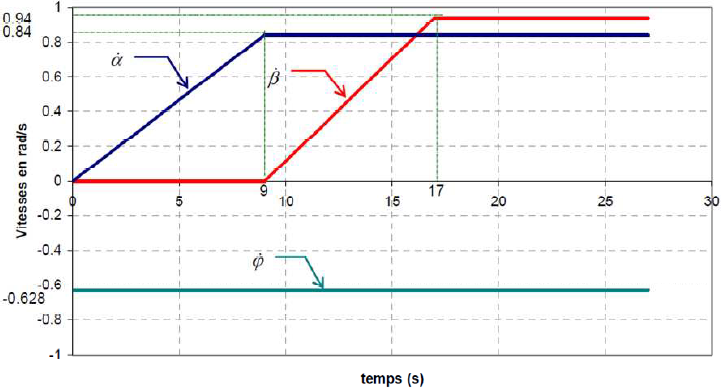
\includegraphics[width=\linewidth]{images/img2}
\end{center}

\subparagraph{\label{lab}}
\textit{Déterminer les valeurs des paramètres $\dot{\alpha}$, $\dot{\beta}$ et $\dot{\varphi}$
puis l'expression analytique des positions angulaires $\alpha(t)$ et $\beta(t)$ et $\varphi(t)$ dans l'intervalle de temps $[17;27]$ secondes en sachant qu'à l'instant $t=\SI{17}{s}$, on a $\alpha=\SI{10,5}{rad}$, $\beta=\SI{3,76}{rad}$ et $\varphi=-\SI{10,676}{rad}$.}
\ifprof
\begin{corrige}

Dans l'intervalle de temps compris entre 17 et 27 secondes, les vitesses angulaires sont constantes.

$$
\systeq{
{\dot\alpha}{=\SI{0,84}{rad/s}}\\
{\dot\beta}{=\SI{0,94}{rad/s}}\\
{\dot\varphi}{=-\SI{0,628}{rad/s}}
}
$$

Ainsi, par intégration :
\begin{align*}
\alpha (t)-\alpha(17)&=\int_{17}^t \dot\alpha d\tau \\
%\alpha (t)-10,5&=0,84(t-17) \\
%{\alpha (t) }{= 0,84(t-17) + 10,5}\\	
%\beta (t)-\beta(17)&=\int_{17}^t \dot\beta d\tau \\
%\beta (t)-3,76&=0,94(t-17) \\
%{\beta (t) }{= 0,94(t-17) + 3,76}	\\
%\varphi (t)-\varphi(17)&=\int_{17}^t \dot\varphi d\tau \\
%\varphi (t)+10,676&=-0,628(t-17) \\
%{\varphi (t) }{= -0,628(t-17) -10,676}	\\
\end{align*}
\end{corrige}\else\fi

\subparagraph{}
\textit{Déterminer les valeurs numériques à l'instant $t_1=19,8\; s$ de $\alpha$, $\beta$ et $\varphi$.}
\ifprof
\begin{corrige}

Pour $t=19,8$ s,
\[
\systeq{
\alpha&=0,84 \times (19,8-17) + 10,5=\boxed{12,85\text{ rad}}\\
\beta&=0,94\times (19,8-17) +3,76 = \boxed{6,39\text{ rad}}\\
\varphi &= -0,628\times (19,8-17) -10,676 =\boxed{12,43\text{ rad}}
}
\]

\end{corrige}\else\fi

\subparagraph{}
\textit{On pose $\vectv{P}{3}{0}=V_{x2}\vect{x_2}+V_{y2}\vect{y_2}+V_{z2}\vect{z_2}$. Déterminer les expressions littérales de $V_{x2}$, $V_{x2}$, $V_{z2}$ puis les valeurs numériques de à $t_1=19,8\;s.$} (On donne : $l_1=3,9\;m$, $l_2=2,87\;m$, $R=2,61\;m$.)
\ifprof
\begin{corrige}

Il s'agit de projeter le vecteur \vecvit{P}{3}{0} dans la base $(\vect{x_2}, \vect{y_2} ,\vect{z_0})$. En effet, le vecteur $\vect{z_2}$ est identique au vecteur $\vect{z_0}$.
\begin{align*}
\vecvit{P}{3}{0}&=V_{x2}\vect{x_2} +V_{y2}\vect{y_2} + V_{z2}\vect{z_0}\\
V_{x2}&=\vecvit{P}{3}{0}\cdot\vect{x_2}\\
	&=\left(l_1\dot\alpha\vx1+l_2(\dot\alpha+\dot\beta)\vect{x_2}-R\sin\varphi(\dot\alpha+\dot\beta)\vect{y_2}-R\dot\varphi\vect{x_3}\right)\cdot\vect{x_2}\\
{V_{x2}}{=l_1 \dot\alpha\cos\beta+l_2 (\dot\alpha+\dot\beta) -R \dot\varphi\cos\varphi}\\
V_{y2}&=\vecvit{P}{3}{0}\cdot\vect{y_2}\\
	&=\left(l_1\dot\alpha\vx1+l_2(\dot\alpha+\dot\beta)\vect{x_2}-R\sin\varphi(\dot\alpha+\dot\beta)\vect{y_2}-R\dot\varphi\vect{x_3}\right)\cdot\vect{y_2}\\
{V_{y2}}{=-l_1\dot\alpha\sin\beta-R\sin\varphi(\dot\alpha+\dot\beta)}\\
V_{z2}&=\vecvit{P}{3}{0}\cdot\vect{y_2}\\
	&=\left(l_1\dot\alpha\vx1+l_2(\dot\alpha+\dot\beta)\vect{x_2}-R\sin\varphi(\dot\alpha+\dot\beta)\vect{y_2}-R\dot\varphi\vect{x_3}\right)\cdot\vect{z_0}\\
{V_{z2}}{=R\dot\varphi\sin\varphi}
\end{align*}

Valeurs numériques à $t=19,8$ s :

\begin{align*}
V_{x2}&=3,9\times 0,84 \times \cos (6,39) + 2,87  \times (0,84 + 0,94) + 2,61 \times 0,628 \times \cos (12,43) \\
	&=\boxed{9,99\text{ m/s}}\\
V_{y2}&=-3,9 \times 0,84 \times \sin(6,39) - 2,61 \times \sin(12,43) \times (0,84 + 0,94)\\
	&=\boxed{-0,28\text{ m/s}}\\
V_{z2}&=-2,61\times 0,628 \times \sin(12,43) \\
	&=\boxed{-0,22 \text{ m/s}}
\end{align*}

\end{corrige}\else\fi

\subparagraph{}
\textit{Calculer $\vect{\Gamma\left(P\in3/0 \right)}$.}
\ifprof
\begin{corrige}

\begin{align*}
\vecacc{P}{3}{0}&=\gderivect{\vecvit{P}{3}{0}}{0}\\
	&=\dfrac{\dd}{\dd t}\left( l_1\dot\alpha\vx1+l_2(\dot\alpha+\dot\beta)\vect{x_2}-R\sin\varphi(\dot\alpha+\dot\beta)\vect{y_2}-R\dot\varphi\vect{x_3} \right)_0 \\
	&=l_1 \ddot\alpha\vx1+l_1 \dot\alpha\underbrace{\derivect{\vx1}{0}}_{\dot\alpha\vy1} + l_2(\ddot\alpha + \ddot\beta)\vect{x_2}+ l_2(\dot\alpha+\dot\beta)\underbrace{\derivect{\vect{x_2}}{0}}_{(\dot\alpha+\dot\beta)\vect{y_2}}-R\dot\varphi\cos\varphi(\dot\alpha+\dot\beta)\vect{y_2}\\
	&\phantom{==}-R\sin\varphi(\ddot\alpha+\ddot\beta)\vect{y_2}-R\sin\varphi(\dot\alpha+\dot\beta)\underbrace{\derivect{\vect{y_2}}{0}}_{-(\dot\alpha+\dot\beta)\vect{x_2}}-R\ddot\varphi\vect{x_3} -R\dot\varphi\derivect{\vect{x_3}}{0}\\
\derivect{\vect{x_3}}{0}&={\derivect{\vect{x_3}}{3}}+\vecrot{3}{0}\wedge\vect{x_3}\\
		&=\left((\dot\alpha+\dot\beta)\vect{z_0}+\dot\varphi\vect{y_2}\right)\wedge\vect{x_3}\\
		&=(\dot\alpha+\dot\beta)\cos\varphi\vect{y_2}-\dot\varphi\vect{z_3}
		\end{align*}
		
D'où :
\begin{align*}
\vecacc{P}{3}{0}&=l_1 \ddot\alpha\vx1+l_1 \dot\alpha^2\vy1 + l_2(\ddot\alpha + \ddot\beta)\vect{x_2}+ l_2(\dot\alpha+\dot\beta)^2\vect{y_2}-2R\dot\varphi\cos\varphi(\dot\alpha+\dot\beta)\vect{y_2}\\
	& -R\sin\varphi(\ddot\alpha+\ddot\beta)\vect{y_2}+R\sin\varphi(\dot\alpha+\dot\beta)^2\vect{x_2}-R\ddot\varphi\vect{x_3} +R\dot\varphi^2\vect{z_3}
\end{align*}


\end{corrige}\else\fi

\subparagraph{}
\textit{Calculer $\vect{\Gamma\left(P\in3/0 \right)}$ dans l'intervalle de temps $[17;27]$ secondes pour lequel les vitesses angulaires sont constantes.}
\ifprof
\begin{corrige}

Dans le cas ou les vitesses angulaires sont constantes, les accélérations angulaires $\ddot\alpha$, $\ddot\beta$, et $\ddot\varphi$ sont nulles. L'expression de \vecacc{P}{3}{0} se simplifie donc :
\begin{align*}
{\vecacc{P}{3}{0}}{=l_1 \dot\alpha^2\vy1 + l_2(\dot\alpha+\dot\beta)^2\vect{y_2}-2R\dot\varphi\cos\varphi(\dot\alpha+\dot\beta)\vect{y_2}+ R\sin\varphi(\dot\alpha+\dot\beta)^2\vect{x_2} +R\dot\varphi^2\vect{z_3}}\\
\end{align*}

\end{corrige}\else\fi

\vspace{.3cm}

Le graphe ci-dessous, obtenu par simulation numérique, présente le module de la vitesse du passager $P$ par rapport au bâti 0 ainsi que le module de l'accélération du passager $P$ par rapport au bâti 0 en fonction du temps. 
\begin{center}
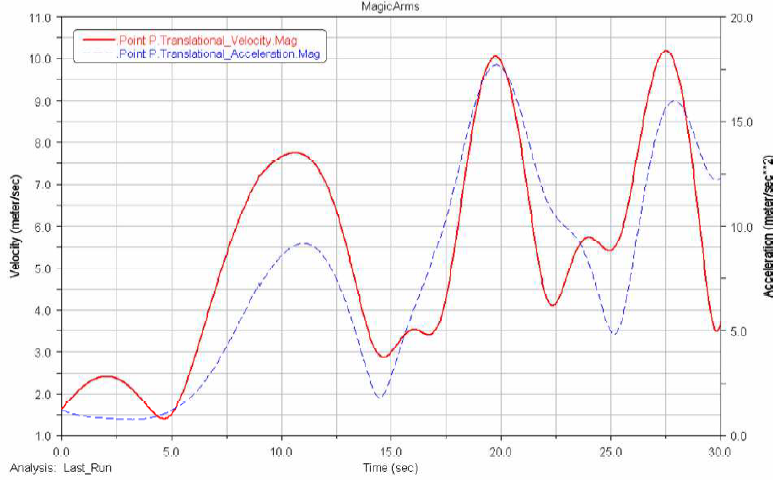
\includegraphics[width=\linewidth]{images/img3}
\end{center}

\subparagraph{}
\textit{Comparer les résultats obtenus à la question \ref{lab} à ceux du graphe pour le temps $t_1=19,8\;s.$.}
\ifprof
\begin{corrige}

Le graphe montre qu'à $t=19,8$ s, l'intensité du vecteur \vecvit{P}{3}{0} vaut 10 m/s. Or  d'après la question~8, 
\begin{align*}
\left|\left|\vecvit{P}{3}{0}\right|\right|&=\sqrt{V_{x2}^2+V_{y2}^2+V_{z2}^2}\\
	&=\sqrt{9,99^2+0,28^2+0,22^2}\\
	&=\boxed{10\text{ m/s} }
\end{align*}

On constate que le calcul littéral nous donne le même résultat que l'exploitation de la courbe.

\end{corrige}\else\fi

\subparagraph{}
\textit{Relever l'accélération maximale subie par le passager et conclure vis-à-vis du CdCF.}
\ifprof
\begin{corrige}
D'après la courbe de l'accélération (en pointillés), la valeur maximale de l'accélération subie par le passager vaut 17,5 m/s\up{2}. Le cahier des charges exige que l'accélération maximale ne dépasse pas 2,5 $g$, soit 24,5 m/s\up{2}. Le cahier des charges est donc respecté.

\end{corrige}\else\fi



\begin{enumerate}
\item $\;$
\item $\vecrot{1}{0}=\dot\alpha\vect{z_0}$, $\vecrot{2}{1}=\dot\beta\vect{z_0}$, $\vecrot{3}{2}=\dot\varphi\vect{y_2}$.
\item $\vecrot{2}{0}=(\dot\alpha+\dot\beta)\vect{z_0}$, $\vecrot{3}{0}=(\dot\alpha+\dot\beta)\vect{z_0}+\dot\varphi\vect{y_2}$;
\item 
$\vect{z_2} \wedge \vect{z_3} =\sin\varphi \vect{y_2}$,
$\vect{x_3} \wedge \vect{x_2} = -\sin\varphi \vect{y_2}$,
$\vect{x_3} \wedge \vect{z_2}=-\cos\varphi\vect{y_2}$,
$\vect{z_2} \wedge \vect{z_1}= \vec{0}$,
$\vect{x_2} \wedge \vect{x_0}=-\sin(\beta+\alpha)\vect{z_0}$,
$\vect{x_3}\wedge\vect{z_0} =-\cos\varphi\vect{y_2}$.
\item 
${\vecvit{O_2}{2}{0}}{= l_1\dot\alpha\vx1}$,
${\vecvit{O_3}{3}{0}}{=l_1\dot\alpha\vx1+l_2(\dot\alpha+\dot\beta)\vect{x_2}}$,
${\vecvit{P}{3}{0}}{=l_1\dot\alpha\vx1+l_2(\dot\alpha+\dot\beta)\vect{x_2}-R\sin\varphi(\dot\alpha+\dot\beta)\vect{y_2}-R\dot\varphi\vect{x_3}}$.

\item ${\dot\alpha}{=\SI{0,84}{rad/s}}$, ${\dot\beta}{=\SI{0,94}{rad/s}}$, ${\dot\varphi}{=-\SI{0,628}{rad/s}}$ et $\alpha (t)-\alpha(17)=\int_{17}^t \dot\alpha d\tau$.
\item $\alpha=\boxed{12,85\text{ rad}}$, $\beta= \boxed{6,39\text{ rad}}$, $\varphi = \boxed{12,43\text{ rad}}$.
\item ${V_{x2}}{=l_1 \dot\alpha\cos\beta+l_2 (\dot\alpha+\dot\beta) -R \dot\varphi\cos\varphi}=\boxed{9,99\text{ m/s}}$, 
${V_{y2}}{=-l_1\dot\alpha\sin\beta-R\sin\varphi(\dot\alpha+\dot\beta)}=\boxed{-0,28\text{ m/s}}$,
$ {V_{z2}}{=R\dot\varphi\sin\varphi} =\boxed{-0,22 \text{ m/s}}$.

\item $\vecacc{P}{3}{0}=l_1 \ddot\alpha\vx1+l_1 \dot\alpha^2\vy1 + l_2(\ddot\alpha + \ddot\beta)\vect{x_2}+ l_2(\dot\alpha+\dot\beta)^2\vect{y_2}-2R\dot\varphi\cos\varphi(\dot\alpha+\dot\beta)\vect{y_2} -R\sin\varphi(\ddot\alpha+\ddot\beta)\vect{y_2}+R\sin\varphi(\dot\alpha+\dot\beta)^2\vect{x_2}-R\ddot\varphi\vect{x_3} +R\dot\varphi^2\vect{z_3}$.

\item ${\vecacc{P}{3}{0}}=l_1 \dot\alpha^2\vect{y_1} + l_2(\dot\alpha+\dot\beta)^2\vect{y_2}-2R\dot\varphi\cos\varphi(\dot\alpha+\dot\beta)\vect{y_2}+ R\sin\varphi(\dot\alpha+\dot\beta)^2\vect{x_2} +R\dot\varphi^2\vect{z_3}$.

\item $\left|\left|\vecvit{P}{3}{0}\right|\right|=\boxed{10\text{ m/s}}$

\item $ \quad$.

\end{enumerate}


\ifprof
\else
\end{multicols}
\fi


%\begin{center}
%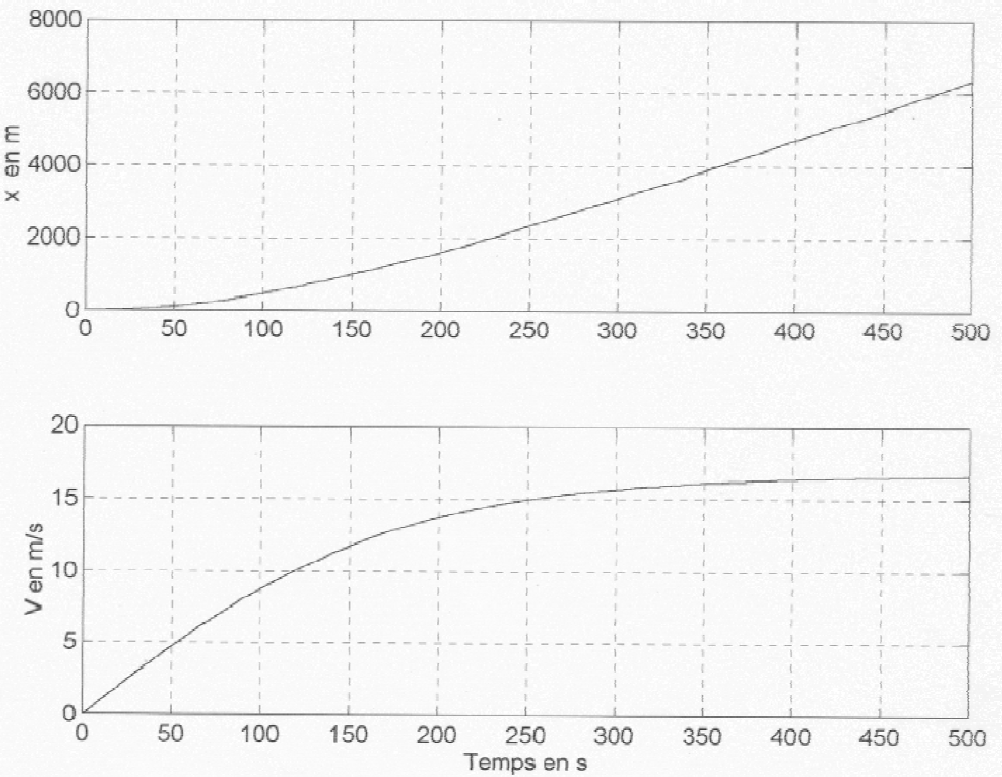
\includegraphics[width=\linewidth]{images/fig_04}
%%\textit{}
%\end{center}

\end{document}

\subparagraph{}\textit{}


\begin{center}
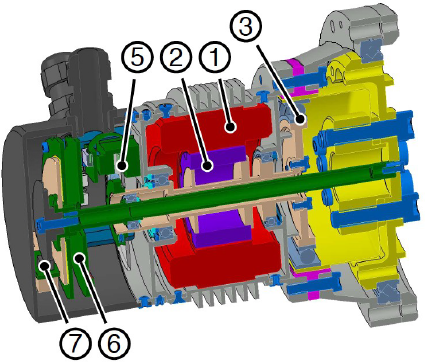
\includegraphics[width=\linewidth]{images/fig_06}
%\textit{}
\end{center}
\begin{center}
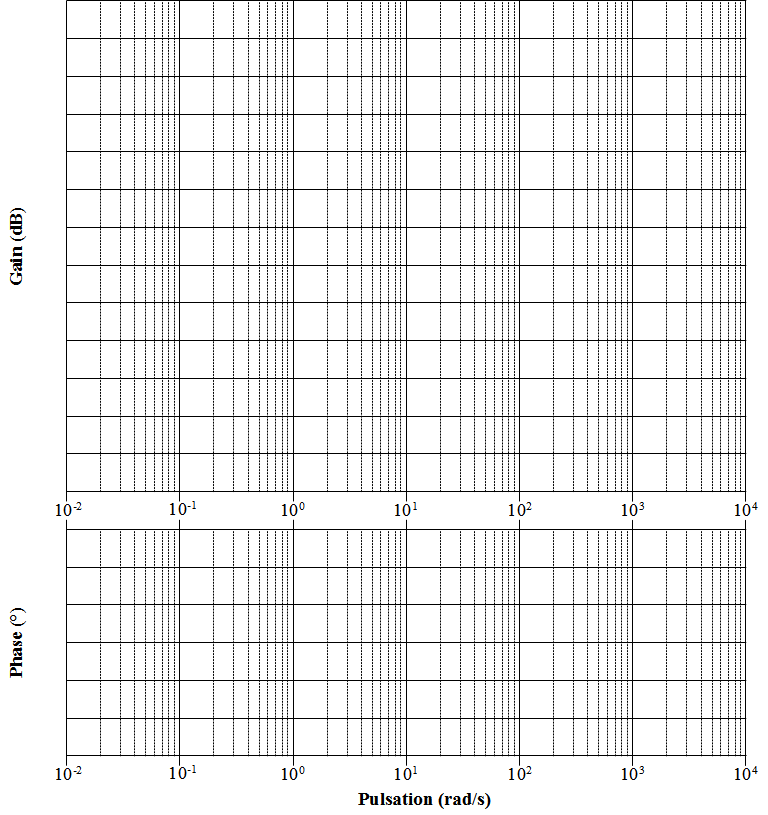
\includegraphics[width=\linewidth]{images/img_04}
%\textit{}
\end{center}



%%%%%%%%%%%%%%%%%%%%%%%%%%%%
